% ==============================================================================
% Spatial Dynamics of Disappearances in Mexico, 2015–2025
% Target: Journal of Quantitative Criminology (JQC), Springer
% Monthly pipeline — Paper 1 of series
% ==============================================================================

\documentclass[12pt]{article}

% ---- Packages ----------------------------------------------------------------
\usepackage[margin=1in]{geometry}
\usepackage{booktabs}
\usepackage{graphicx}
\usepackage{amsmath}
\usepackage{natbib}
\usepackage{setspace}
\usepackage[colorlinks=true,linkcolor=blue,citecolor=blue,urlcolor=blue]{hyperref}
\usepackage[font=small,labelfont=bf]{caption}
\usepackage{subcaption}
\usepackage{adjustbox}
\usepackage{array}
\usepackage{xcolor}

% ---- TODO system -------------------------------------------------------------
\newcommand{\todo}[1]{\textcolor{red}{\textbf{[TODO: #1]}}}
\newcommand{\todoverify}[1]{\textcolor{orange}{\textbf{[VERIFY: #1]}}}
\newcommand{\todocite}[1]{\textcolor{blue}{\textbf{[CITE: #1]}}}
\newcommand{\todowrite}[1]{\textcolor{purple}{\textbf{[WRITE: #1]}}}

% ---- Study parameter commands ------------------------------------------------
\newcommand{\studyperiod}{January 2015 -- December 2025}
\newcommand{\nmonths}{132}
\newcommand{\nmunis}{2,478}
\newcommand{\referencemonth}{June 2025}
\newcommand{\bookendstart}{June 2015}
\newcommand{\nislands}{0}
\newcommand{\nLISAruns}{1,584}

% ---- Document settings -------------------------------------------------------
\doublespacing

% ---- Metadata ----------------------------------------------------------------
\title{Spatial Dynamics of Disappearances in Mexico, 2015--2025:\\
       A Municipal-Level Analysis by Outcome Status}

\author{Marco A.\ Escobar\textsuperscript{1} \and
        Gerardo Reyes-Guzman\textsuperscript{2} \and
        Abraham Sanchez Ruiz\textsuperscript{3} \\[6pt]
        \small\textsuperscript{1}\todo{Affiliation 1} \\
        \small\textsuperscript{2}\todo{Affiliation 2} \\
        \small\textsuperscript{3}\todo{Affiliation 3}}
\date{\today}

% ==============================================================================
\begin{document}
\maketitle

% ---- Abstract ----------------------------------------------------------------
% ==============================================================================
% Abstract (structured per JQC requirements)
% ==============================================================================
\begin{abstract}
\noindent\textbf{Objectives.}
Prior spatial analyses of disappearances in Mexico treat them as a single phenomenon.
We present the first outcome-disaggregated spatial analysis, examining whether four outcome statuses---Not Located, Located Alive, Located Dead, and Total---produce distinct hotspot geographies.

\noindent\textbf{Methods.}
We analyze \nmunis{} municipalities over \nmonths{} months (January 2015--December 2025) using Local Indicators of Spatial Association (LISA) with Queen contiguity weights (\nLISAruns{} runs: 4 statuses $\times$ 3 sexes $\times$ \nmonths{} months).
Geographic concentration is measured via Gini coefficients benchmarked against the law of crime concentration.
Cross-status spatial overlap is quantified using Jaccard similarity on pairwise High-High cluster sets.
Trend slopes use Newey-West HAC standard errors.

\noindent\textbf{Results.}
Outcome statuses are spatially non-interchangeable: Jaccard similarity between Located Dead and Not Located hotspots is 0.143; between Located Dead and Located Alive, 0.151.
Concentration exceeds the Weisburd benchmark two- to threefold: 50\% of Not Located cases concentrate in 42 municipalities (1.7\%).
Centro is the fastest-growing cluster region (Not Located: $+4.96$ municipalities/year, $p < 0.001$), invisible to prior annual analyses.
The ``rising Baj\'{i}o'' hypothesis is rejected (Total: $-1.09$/year, $p = 0.024$).
Sex disaggregation reveals divergent male/female hotspot geographies for Not Located (Jaccard = 0.262) and a power failure for female Located Dead (zero HH municipalities).
Findings align with the UN Committee on Enforced Disappearances' 2026 characterization of spatially heterogeneous attacks.

\noindent\textbf{Conclusions.}
Forensic and prevention resources require different geographic targeting: Located Dead hotspots and Not Located hotspots are different places.
Composite disappearance maps conflating all statuses misallocate resources toward Located Alive--dominated geographies.
\end{abstract}


\textbf{Keywords:} enforced disappearances; spatial autocorrelation; LISA;
Mexico; outcome status; municipal level; hotspot analysis; crime concentration

\newpage

% ==============================================================================
% ==============================================================================
% Section 1: Introduction
% ==============================================================================
\section{Introduction}
\label{sec:intro}

% ---- Block 1: Scale and stakes ------------------------------------------------
Mexico's disappearance crisis is among the most severe humanitarian emergencies in the Western Hemisphere.
As of early 2026, the Registro Nacional de Personas Desaparecidas y No Localizadas (RNPDNO) has recorded over 115,000 persons whose whereabouts remain unknown---a figure widely acknowledged to undercount the true scale \citep{mandolessi_2022, guercke_2021}.
In March 2026, the UN Committee on Enforced Disappearances (CED) issued its first-ever referral to the General Assembly under Article~34 of the Convention, finding that enforced disappearances in Mexico constitute crimes against humanity \citep{CED_MEX_art34_2026}.
The decision explicitly notes that attacks occurred ``at different moments and in different parts of the territory''---a spatial and temporal characterization that, until now, has lacked systematic quantitative support at the national scale.
Forced disappearances have been documented across multiple contexts: as a tool of state repression, a byproduct of organized criminal violence, and a consequence of weak institutional capacity to investigate and resolve cases \citep{solar_2021, guercke_2021, rios_2013}.

% ---- Block 2: Spatial criminology lineage --------------------------------------
Spatial analysis of crime has a well-established lineage in quantitative criminology.
\citet{sherman_1989} demonstrated that predatory crime concentrates at specific places, a finding that launched the hot-spot policing paradigm \citep{braga_hotspots_2014}.
\citet{anselin_1995}'s Local Indicators of Spatial Association (LISA) provided the statistical framework for identifying clusters of high and low values while accounting for spatial dependence.
\citet{weisburd_2015}'s ``law of crime concentration'' formalized the empirical regularity that approximately 50\% of crime occurs in 4--6\% of places, a benchmark that has been validated across cities and crime types \citep{weisburd_2004, curman_2015, steenbeek_weisburd_2016}.
The \emph{Journal of Quantitative Criminology} has dedicated special issues to place-based crime analysis \citep{braga_law_2017, andresen_advances_2021}, and concentration measurement has been refined using Gini coefficients and related indices \citep{prieto_curiel_2018, schnell_braga_piza_2017}.

% ---- Block 3: Mexico-specific spatial work -------------------------------------
Spatial analysis of violence in Mexico has focused primarily on homicides.
\citet{vilalta_muggah_2016} and \citet{vilalta_2021} examined homicide patterns in Mexico City using spatial regression and diffusion models, identifying neighborhood-level clustering tied to socioeconomic deprivation and routine activities.
\citet{cadena_garrocho_2019} provided the first national-scale spatial analysis to include both homicides and disappearances at the municipal level for 2006--2017, documenting a northward shift in violence associated with cartel territorial competition---but treated disappearances as a monolithic category.
\citet{atuesta_2024} examined organized crime-related disappearances in three northern states (Durango, Tamaulipas, Coahuila) using case-level data, documenting spatial patterns linked to drug trafficking routes, but their analysis was restricted to three states and did not examine outcome status decomposition.
\citet{aguilar_velazquez_2025} analyzed disappearances in Mexico City using data-driven methods but at a single-city scale.
None of these studies disaggregated disappearances by outcome status or examined the full national territory at monthly resolution.

% ---- Block 4: The gap ---------------------------------------------------------
All prior spatial work on disappearances in Mexico treats them as a single phenomenon.
This is a consequential simplification.
The RNPDNO distinguishes four outcome statuses that reflect fundamentally different processes: Not Located cases represent active search failures---persons whose whereabouts remain unknown; Located Alive cases represent successful recoveries; and Located Dead cases represent lethal outcomes.
If these processes are driven by different actors, institutional responses, or structural conditions, they should produce different spatial signatures.
A municipality that is a hotspot for living recoveries may not be a hotspot for lethal outcomes; a municipality with many unresolved cases may not be a municipality where bodies are found.
These distinctions have direct implications for resource allocation: forensic identification teams should be deployed where lethal outcomes concentrate, while active search and prevention programs should target areas of concentrated unresolved cases---and these may be different places.
The RNPDNO makes outcome-disaggregated analysis possible, but no study has exploited this structure at the national scale.

% ---- Block 5: This paper -------------------------------------------------------
This paper presents the first outcome-disaggregated spatial analysis of disappearances in Mexico at the national scale with monthly resolution.
We analyze \nmunis{} municipalities over \nmonths{} months (\studyperiod{}) across four outcome statuses, executing \nLISAruns{} LISA runs.
Two methodological contributions distinguish this work.
First, we quantify cross-status spatial non-interchangeability using Jaccard similarity coefficients on pairwise HH cluster sets---demonstrating that outcome statuses produce distinct hotspot geographies.
Second, the monthly temporal resolution reveals dynamics invisible to annual analyses, most notably the rapid expansion of HH clusters in Mexico's Centro region.
We further examine whether the CED's qualitative geographic claims about eight named states find support in the quantitative spatial record.
A companion Data in Brief descriptor documents the dataset schema and processing pipeline \citep{escobar_rnpdno_2026}.

% ---- Block 6: Research questions -----------------------------------------------
This paper addresses four research questions:

\begin{enumerate}
  \item \textbf{RQ1 (Concentration):} How geographically concentrated are
        disappearances, and does concentration differ across outcome statuses?
  \item \textbf{RQ2 (Clustering):} Do the four outcome statuses produce distinct
        spatial cluster geographies at the municipal level?
  \item \textbf{RQ3 (Temporal dynamics):} How has the spatial distribution of
        each status evolved from 2015 to 2025, and do regional hotspot trajectories
        diverge by outcome?
  \item \textbf{RQ4 (Sex disaggregation):} Do male and female disappearances
        exhibit different spatial patterns across outcome statuses?
\end{enumerate}

\noindent We additionally examine the alignment between our empirical findings and the CED's geographic characterization of disappearance patterns across eight named states.


% ==============================================================================
\section{Data}
\label{sec:data}
\subsection{National Registry of Disappeared and Not Located Persons}

The National Registry of Missing and Unlocated Persons (\textit{Registro Nacional de Personas Desaparecidas y No Localizadas}, RNPDNO) is Mexico's centralized registry of disappearance cases, established under the 2017 General Law on Disappearances \citep{ley_general_2017} and administered by the National Search Commission (\textit{Comisión Nacional de Búsqueda}, CNB). The CNB publishes aggregate statistics and visualizations through a public dashboard \citep{cnb_rnpdno} but does not release machine-readable, municipality-level data files. The dataset used in this study was constructed by web-scraping, geocoding, and processing the dashboard records into four structured CSV files, one per outcome status \citep{escobar_rnpdno_2026}.

The registry records new disappearance cases each month, not a running total of all cases since the registry was created. During the \nmonths{}-month study period \studyperiod{}, the registry recorded 263,402 person-registrations, of which 89,631 were classified as Not Located, 157,990 as Located Alive, and 15,438 as Located Dead (Table~\ref{tab:dataset}). Municipality-month combinations with no recorded cases are treated as zero registrations, yielding a balanced panel of \nmunis{} municipalities observed over \nmonths{} months and four outcome categories. Records with unresolvable municipality identifiers (12,206 persons, 4.6\% of Total registrations) are excluded from spatial analyses, potentially biasing hotspot maps toward municipalities with more complete geocoding. Each file additionally provides sex-disaggregated counts (male, female, undefined).
\begin{tabular}{lrrrrrrrr}
  \toprule
  & & & & \multicolumn{4}{c}{\textbf{Valid persons (by sex)}} \\
  \cmidrule(lr){5-8}
  \textbf{Status} & \textbf{Valid rows} & \textbf{Sentinel rows} & \textbf{Valid persons} & \textbf{Male} & \textbf{Female} & \textbf{Undef.} & \textbf{\%Male} \\
  \midrule
  Total          & 55,524 & 1,803 & 262,814 & 160,857 & 101,630 & 327 & 61.2\% \\
  Not Located    & 33,384 & 1,256 &  89,850 &  69,871 &  19,843 & 136 & 77.8\% \\
  Located Alive  & 36,521 &   837 & 157,688 &  77,856 &  79,686 & 146 & 49.4\% \\
  Located Dead   &  9,643 &   240 &  15,343 &  13,175 &   2,123 &  45 & 85.9\% \\
  \bottomrule
  \multicolumn{8}{l}{\footnotesize Temporal coverage: January 2015 -- December 2025. Spatial analysis covers 2,478 municipalities (INEGI 2024).} \\
  \multicolumn{8}{l}{\footnotesize Sentinel geocodes (cvegeo ending 998/999 or = 99998) excluded. \%Male computed over valid persons.} \\
  \multicolumn{8}{l}{\footnotesize Located Alive is the only status with near-equal sex distribution (49.4\% male). Located Dead is the most male-skewed (85.9\%).} \\
\end{tabular}


\subsection{Geographic Framework}

We use the INEGI Marco Geoestad\'{i}stico 2025 \citep{inegi_ageeml}, which defines \nmunis{} municipalities in projected coordinates (EPSG:6372, Mexico ITRF2008/LCC).
The five-digit cvegeo code serves as the spatial join key across all datasets; all \nmunis{} municipalities match one-to-one between the geoparquet and the panel dataset (100\% match rate, zero merge failures).
\subsection{Regional Classification}
Municipalities are classified into five macro-regions following the CESOP scheme \citep{mexicoencifras}: Norte, Norte-Occidente, Centro-Norte, Centro, and Sur.
The sixth region, the Baj\'{i}o industrial corridor, is defined independently of the CESOP classification.
\citet{unger_2014} characterized the Baj\'{i}o as a set of economic corridors organized along six highway axes, encompassing over 200 municipalities.
We adopt a narrower operationalization focused on the urbanized industrial core: the 29 municipalities comprising the 10 metropolitan areas and 4 conurbations identified by \citet{medina_fernandez_2023} from the \emph{Sistema Urbano Nacional} 2018 catalog \citep{conapo_sun_2018}, spanning 14 urban entities across 5 states (Aguascalientes, Guanajuato, Michoac\'{a}n, Quer\'{e}taro, and San Luis Potos\'{i}).
This narrower definition isolates the municipalities where industrial activity, population density, and cartel territorial competition converge. The corridor is not mutually exclusive with the five-region scheme; its municipalities also belong to their respective macro-regions.
Section~\ref{sec:trend} reports trend slopes for all six units.

% ==============================================================================
% ==============================================================================
% Section 3: Methods
% ==============================================================================
\section{Methods}
\label{sec:methods}

\subsection{Spatial Weights}
\label{sec:weights}

We construct a Queen contiguity spatial weights matrix for all \nmunis{} municipalities using the \texttt{libpysal} library \citep{rey_pysal_2010}.
To address sub-metre geometry precision gaps in the source geoparquet that would otherwise produce false island municipalities, we employ fuzzy contiguity with a 50-metre buffer (\texttt{fuzzy\_contiguity(buffering=True, buffer=50)}) rather than exact topological intersection.
The matrix is row-standardized.
This approach yields \nislands{} island municipalities---all boundary gaps are resolved by the buffer tolerance.

\subsection{Global Spatial Autocorrelation}
\label{sec:global}

Global Moran's $I$ quantifies the overall degree of spatial clustering:

\begin{equation}
  I = \frac{n}{\sum_i \sum_j w_{ij}}
      \cdot
      \frac{\sum_i \sum_j w_{ij}(x_i - \bar{x})(x_j - \bar{x})}
           {\sum_i (x_i - \bar{x})^2}
  \label{eq:moran}
\end{equation}

\noindent where $x_i$ is the case count in municipality $i$, $w_{ij}$ are row-standardized Queen contiguity weights, and $n = \text{\nmunis{}}$.
Statistical significance is assessed via 999 conditional permutations at $\alpha = 0.05$.

\subsection{Local Spatial Autocorrelation (LISA)}
\label{sec:lisa}

Local Moran's $I_i$ decomposes the global statistic into municipality-level contributions \citep{anselin_1995}:

\begin{equation}
  I_i = \frac{(x_i - \bar{x})}{m_2} \sum_j w_{ij}(x_j - \bar{x}), \quad
  m_2 = \frac{1}{n}\sum_i (x_i - \bar{x})^2
  \label{eq:lisa}
\end{equation}

\noindent Municipalities are classified into five types based on the sign of their local statistic and the significance of their pseudo-$p$-value at $\alpha = 0.05$: High-High (HH), Low-Low (LL), High-Low (HL), Low-High (LH), and Not Significant (NS).
HH municipalities have high counts surrounded by high-count neighbors; LL municipalities have low counts surrounded by low-count neighbors.

We extract connected-component HH clusters via breadth-first search on the Queen adjacency graph, retaining only clusters of three or more contiguous HH municipalities.
LL clusters are retained in tables for completeness but are not interpreted as a substantive finding: the extreme zero-inflation of the count data (77--98\% of municipality-months record zero cases, depending on status) means that LL classification largely identifies municipalities where nothing happened surrounded by municipalities where nothing happened.

The total computational scope is \nLISAruns{} LISA runs: 4 statuses $\times$ 3 sex categories (total, male, female) $\times$ \nmonths{} months, each computed over $N = \text{\nmunis{}}$ municipalities with 999 permutations.

\subsection{Geographic Concentration}
\label{sec:concentration}

We quantify geographic concentration using the Gini coefficient:

\begin{equation}
  G = \frac{2\sum_{i=1}^{n} i \cdot x_{(i)}}{n \sum_{i=1}^{n} x_{(i)}}
      - \frac{n+1}{n}
  \label{eq:gini}
\end{equation}

\noindent and the Herfindahl-Hirschman Index (HHI):

\begin{equation}
  \text{HHI} = \sum_{i=1}^{n} s_i^2, \quad s_i = \frac{x_i}{\sum_j x_j}
  \label{eq:hhi}
\end{equation}

\noindent where $x_{(i)}$ is the $i$-th order statistic of the count distribution.
Both metrics are computed for each of the \nmonths{} monthly cross-sections per status.
We benchmark our concentration estimates against \citet{weisburd_2015}'s ``law of crime concentration,'' which posits that approximately 50\% of crime concentrates in 4--6\% of places.

\subsection{Trend Analysis}
\label{sec:trend}

We fit OLS regressions of the form $y_t = \alpha + \beta t + \varepsilon_t$ separately for each (region $\times$ status) combination, where $y_t$ is the monthly count of HH municipalities and $t = 1, \ldots, \text{\nmonths{}}$.
Slopes are expressed as municipalities per year ($\hat\beta \times 12$).
Because monthly HH counts exhibit serial correlation, standard errors are computed using the \citet{newey_west_1987} heteroskedasticity and autocorrelation consistent (HAC) estimator with a bandwidth of 12 months.

\subsection{Sex Disaggregation}
\label{sec:sex_methods}

LISA is repeated separately for male and female case counts across all statuses and months.
We compare male and female HH geographies using Jaccard similarity (intersection over union of HH municipality sets) for each status at the \referencemonth{} cross-section.
A critical limitation applies to female Located Dead: with a mean of 0.0065 cases per municipality-month and 99.4\% zero cells, the LISA algorithm lacks sufficient spatial variation to detect meaningful clusters.
Female Located Dead results are reported for completeness but should be interpreted with extreme caution.

\subsection{CED Alignment Analysis}
\label{sec:ced_methods}

As a post-hoc exercise, we extract HH dynamics for eight states explicitly named in the Committee on Enforced Disappearances' Article~34 decision \citep{CED_MEX_art34_2026}: Jalisco, Guanajuato, Coahuila, Veracruz, Nayarit, Tabasco, Nuevo Le\'{o}n, and Estado de M\'{e}xico.
For each state, we count the number of municipalities classified as HH in each month, overlay the CED's temporal claims, and compute OLS trend slopes.
No additional LISA runs are required; this analysis operates entirely on the existing \nLISAruns{} runs.


% ==============================================================================
\section{Results}
\label{sec:results}

% ==============================================================================
% Section 4.1: Descriptive Overview
% ==============================================================================
\subsection{Descriptive Overview}
\label{sec:descriptive}

Figure~\ref{fig:timeseries} presents the national monthly time series for each outcome status, disaggregated by sex. A prominent feature of the time series is the sustained increase in registrations across the study period.
National Not Located registrations grew from 275 per month in January 2015 to 1,170 in June 2025, an increase of $+68.2$ cases per year (Newey-West $t = 10.10$, $p < 0.001$).
Located Dead registrations, though smaller in absolute magnitude, nearly tripled from 49 to 144 over the same period ($+8.8$ cases per year, $t = 4.82$, $p < 0.001$).
Located Alive registrations dominate the Total series numerically, contributing 60.0\% of all registrations across the study period, and grew from 790 to 1,788 per month.


\begin{figure}[htbp]
  \centering
  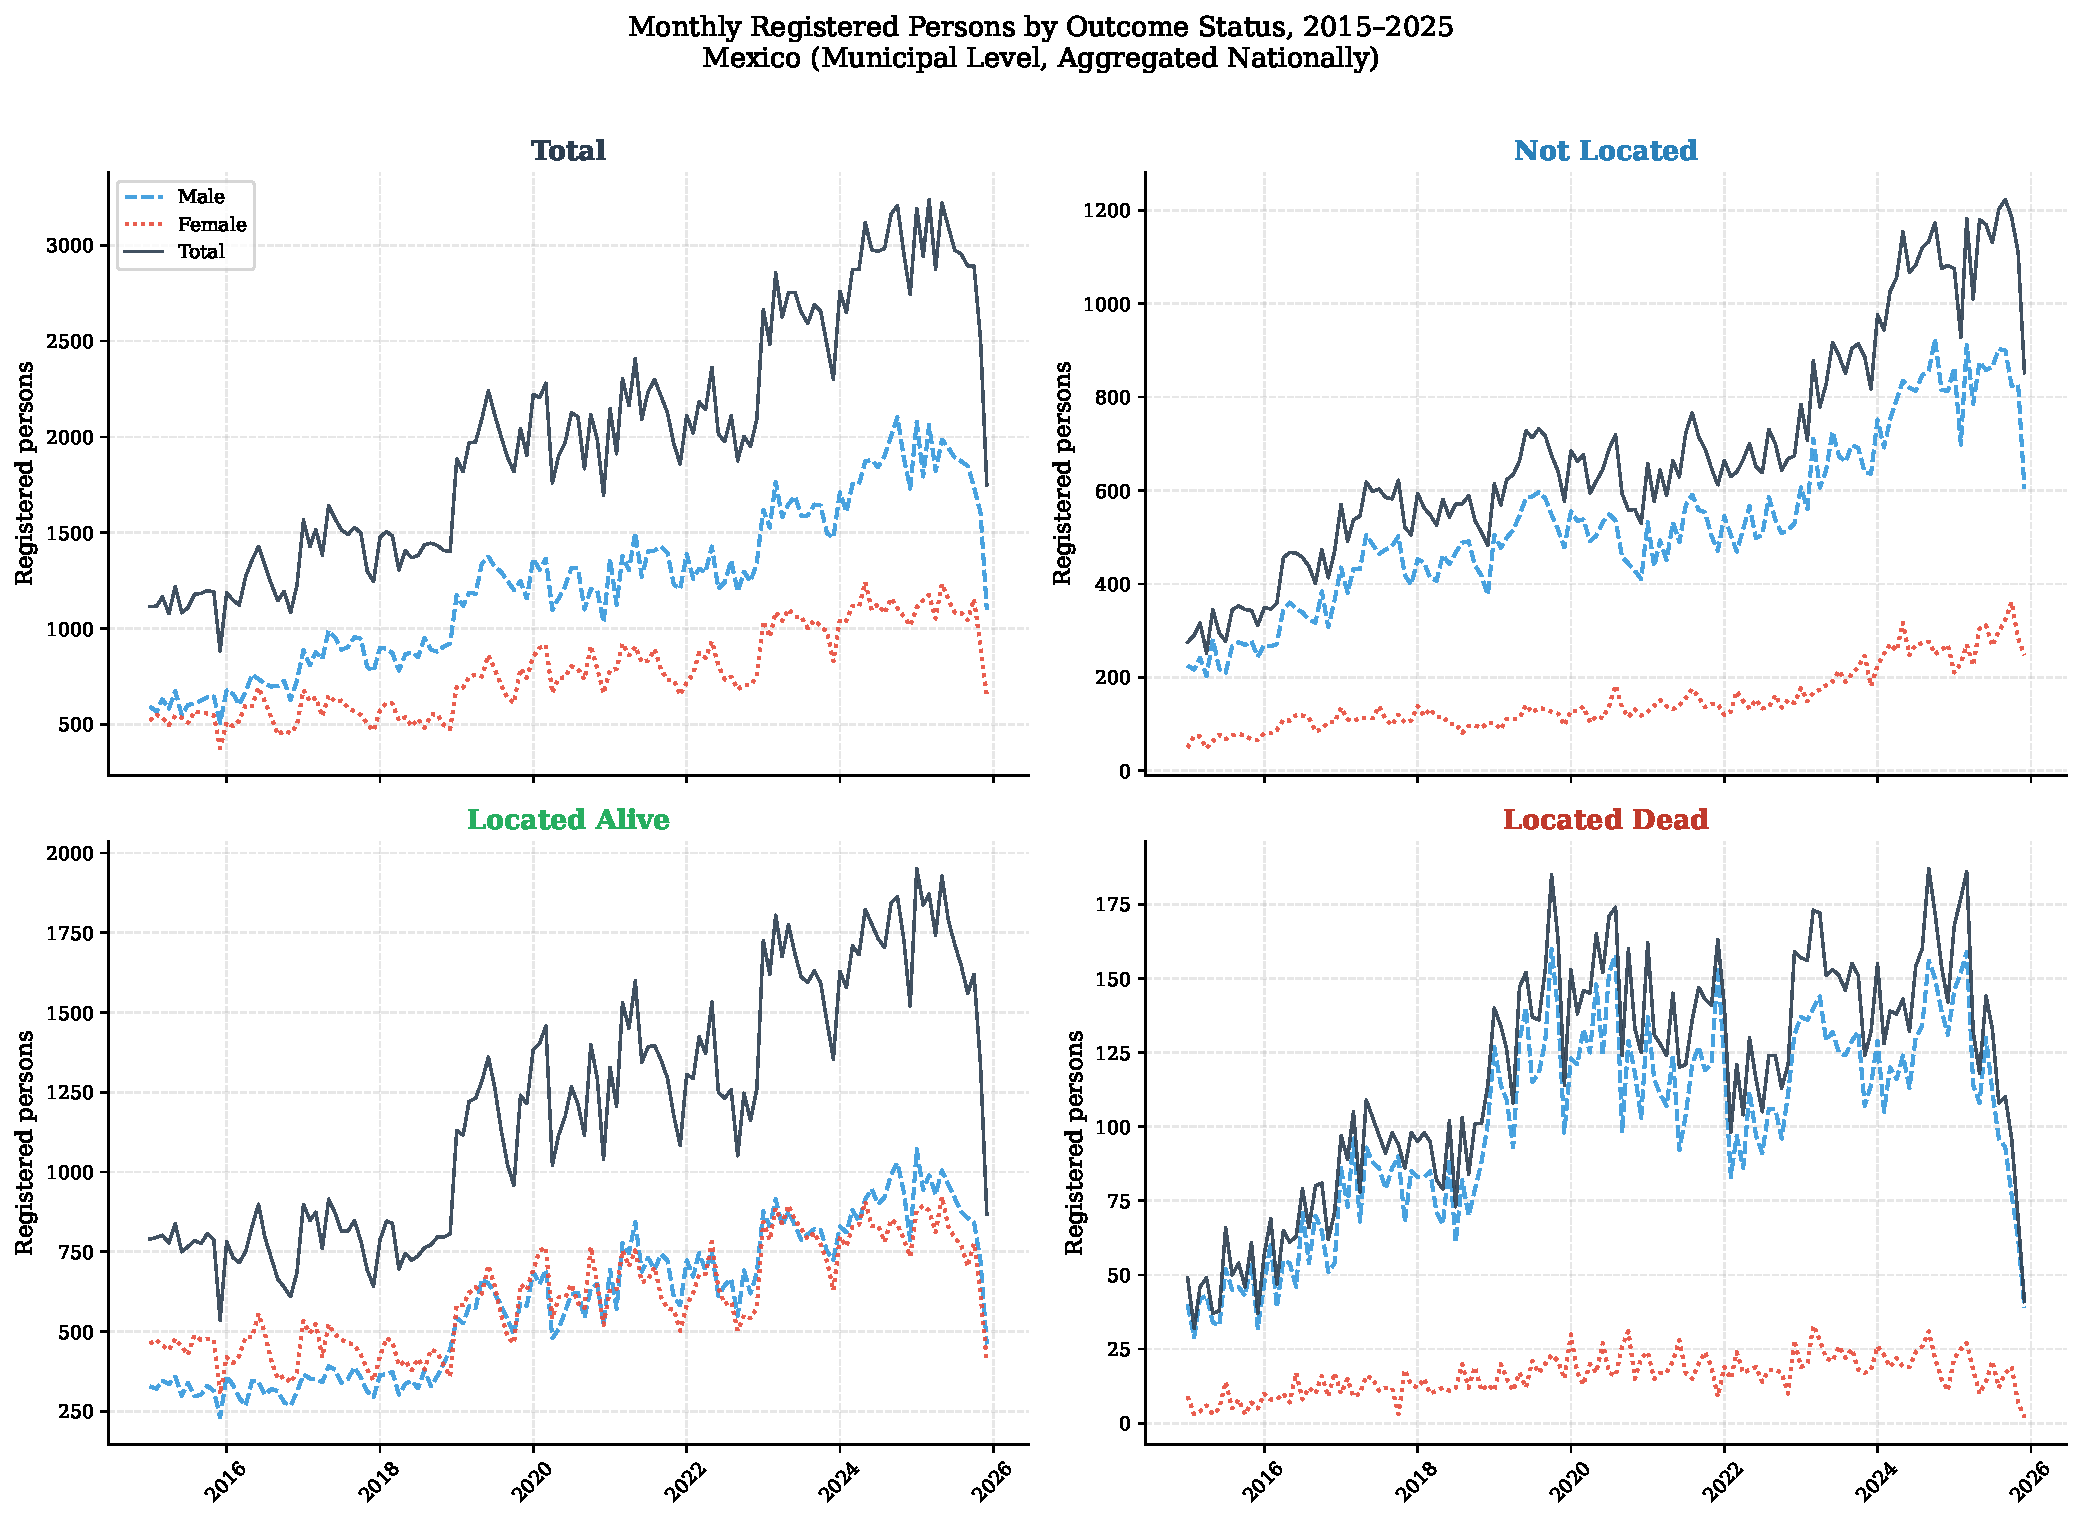
\includegraphics[width=\textwidth]{figures/fig1_time_series_by_status.pdf}
  \caption{Monthly registered persons by outcome status, Mexico, \studyperiod{}.
           Lines show total (solid), male (dashed), and female (dotted)
           case counts aggregated nationally.
           The undefined sex category ($\leq 0.3$\% of registrations) is omitted for clarity.}
  \label{fig:timeseries}
\end{figure}


The sex composition varies markedly across statuses.
Not Located is 77.9\% male, consistent with the established male-dominated profile of disappearance victimization in contexts of organized criminal violence.
Located Dead is even more skewed at 85.9\% male, closely aligned with homicide patterns.
Located Alive, however, approaches near-parity: 49.4\% male and 50.5\% female.
This compositional divergence, where men dominate the population that remains missing while recoveries are gender-balanced, is revisited in Section~\ref{sec:sex}.

Monthly case counts are overwhelmingly zero at the municipality level.
In \referencemonth{}, 77.0\% of municipalities recorded zero Total cases, rising to 85.7\% for Not Located, 84.2\% for Located Alive, and 96.3\% for Located Dead.
All four statuses exhibit extreme right-skew (skewness 11.0 to 21.4): a small number of municipalities contribute disproportionately large counts, a pattern quantified in Section~\ref{sec:concentration_results}.



% ==============================================================================
% Section 4.2: Geographic Concentration (RQ1)
% ==============================================================================
\subsection{Geographic Concentration (RQ1)}
\label{sec:concentration_results}
Across all \nmonths{} months, disappearances are extremely geographically concentrated regardless of outcome status.
The Gini coefficient exceeds 0.91 for every status in every month of the study period (Table~\ref{tab:concentration}).
Located Dead is the most concentrated, with a mean Gini of 0.979 (range: 0.963 to 0.993), followed by Located Alive (mean: 0.955), Not Located (mean: 0.946), and Total (mean: 0.935).

This concentration substantially exceeds standard criminological benchmarks.
\citet{weisburd_2015}'s ``law of crime concentration'' posits that approximately 50\% of crime concentrates in 4 to 6\% of micro-geographic units (street segments).
At the municipal level, concentration is even more pronounced: in \referencemonth{}, 50\% of Not Located registrations concentrate in just 42 municipalities (1.7\% of \nmunis{}), and 50\% of Located Dead registrations in 22 municipalities (0.9\%). Even the least concentrated status, Total, requires only 48 municipalities (1.9\%) to account for half of all registrations.


\begin{figure}[htbp]
  \centering
  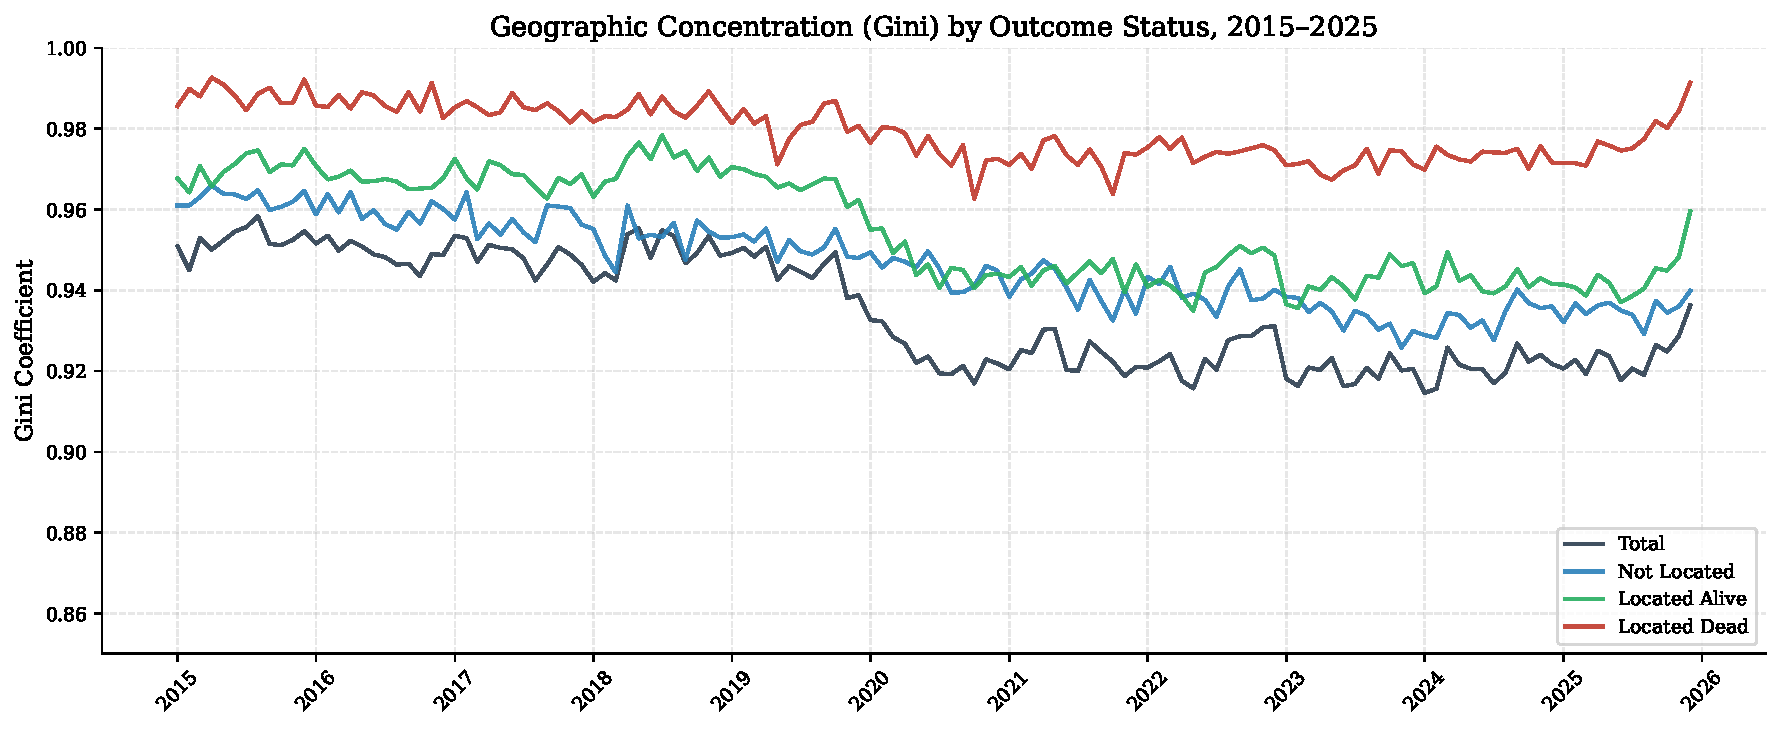
\includegraphics[width=\textwidth]{figures/fig2_gini_time_series.pdf}
  \caption{Gini coefficient of monthly case count distributions by outcome status, \studyperiod{}.
           OLS trend slopes (Gini units per year) annotated.
           Dashed horizontal line indicates Gini = 0.90 reference.}
  \label{fig:gini}
\end{figure}

Despite the extreme levels, all four Gini series exhibit statistically significant negative trends (Figure~\ref{fig:gini}; Table~\ref{tab:concentration}): Total $-0.0038$/yr ($p < 0.001$), Not Located $-0.0032$/yr ($p < 0.001$), Located Alive $-0.0035$/yr ($p < 0.001$), and Located Dead $-0.0017$/yr ($p < 0.001$).
This gradual deconcentration reflects the geographic spread of disappearances into municipalities that previously recorded zero cases: in \bookendstart{}, 88.8\% of municipalities recorded zero Total cases; by \referencemonth{}, this had fallen to 77.0\%.
The deconcentration trend is substantively modest: after a decade of geographic diffusion, concentration remains far above the Weisburd benchmark.

\begin{table}[htbp]
\centering
\caption{Gini coefficient by outcome status, \nmonths{} monthly observations, \studyperiod{}.}\label{tab:concentration}
\begin{tabular}{lrrrr}
  \toprule
  \textbf{Status} & \textbf{Mean} & \textbf{Min} & \textbf{Max} & \textbf{Trend}\tnote{a} \\
  \midrule
  Total         & 0.935 & 0.915 & 0.958 & $-$0.004*** \\
  Not Located   & 0.946 & 0.926 & 0.966 & $-$0.003*** \\
  Located Alive & 0.955 & 0.935 & 0.978 & $-$0.004*** \\
  Located Dead  & 0.979 & 0.963 & 0.993 & $-$0.002*** \\
  \bottomrule
\end{tabular}
\begin{tablenotes}
\small
\item[a] OLS slope per year ($\times$12), 132 monthly observations. $^{***}p<0.001$.
\end{tablenotes}
\end{table}
% ==============================================================================
% Section 4.3: Spatial Clustering (RQ2) — CORE SECTION
% ==============================================================================
\subsection{Spatial Clustering (RQ2)}
\label{sec:clustering}

\subsubsection{Global Spatial Autocorrelation}

Global Moran's $I$ confirms significant positive spatial autocorrelation across virtually the entire study period for all statuses.
Total and Not Located are significant in all 132 months (100\%); Located Alive in 127 of 132 (96.2\%); and Located Dead in 122 of 132 (92.4\%).
The five non-significant months for Located Alive and ten for Located Dead concentrate in the earliest months of the study period, when sparse counts limit statistical power (Figure~\ref{fig:morans}).

\begin{figure}[htbp]
  \centering
  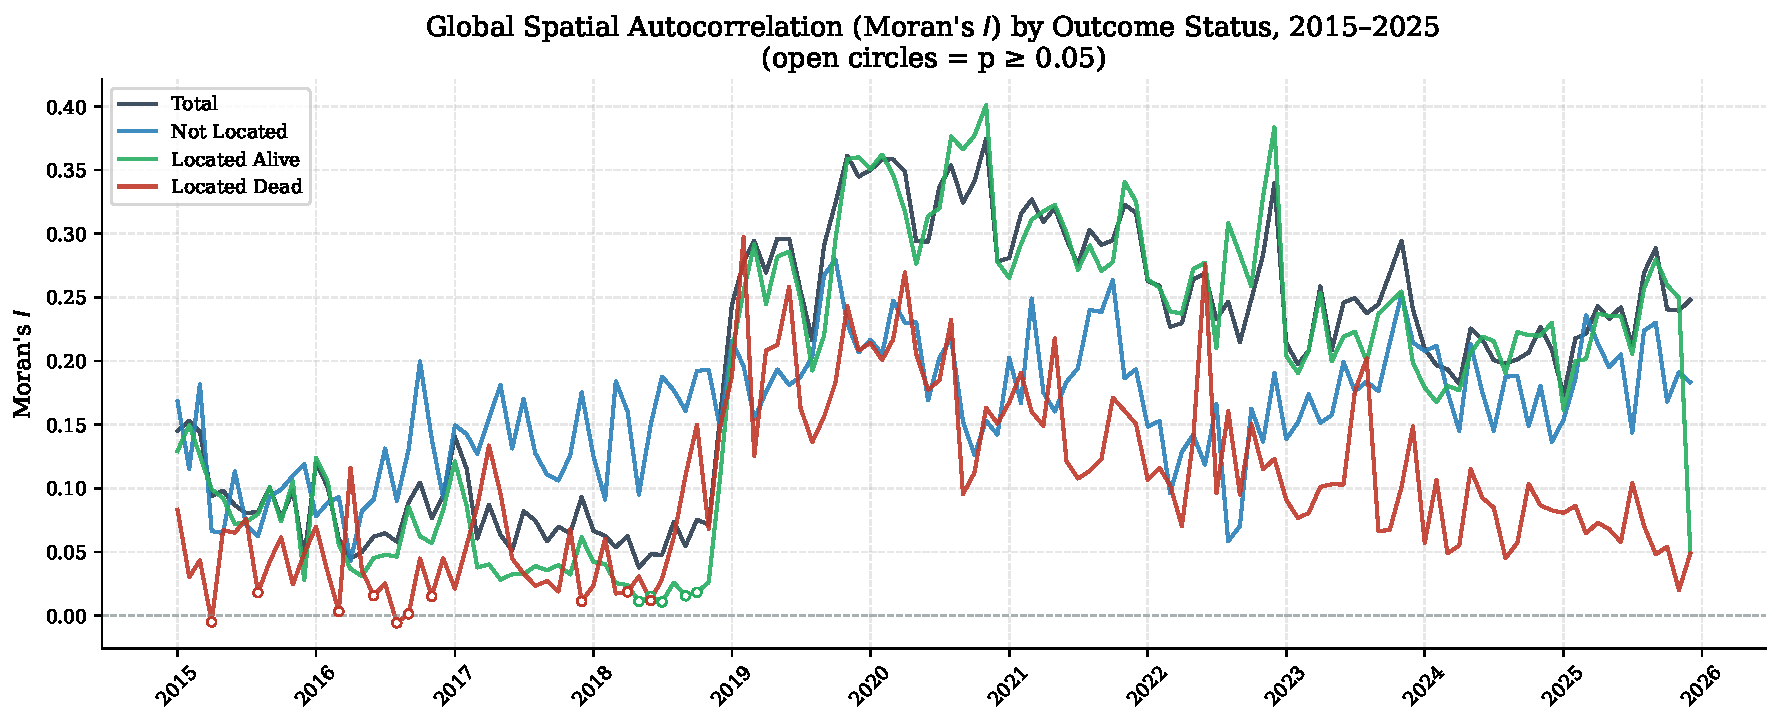
\includegraphics[width=\textwidth]{figures/fig3_morans_i_time_series.pdf}
  \caption{Global Moran's $I$ by outcome status, \studyperiod{}.
           Open circles indicate months with $p \geq 0.05$ (not statistically significant).}
  \label{fig:morans}
\end{figure}

The magnitude of spatial autocorrelation varies by status.
Total shows the highest mean $I$ (0.199, range: 0.038--0.374), followed by Located Alive (0.187, range: 0.011--0.401), Not Located (0.163, range: 0.043--0.280), and Located Dead (0.101, range: $-$0.006--0.298).
The lower values for Located Dead reflect the extreme sparsity of lethal-outcome cases across most of the country.

\subsubsection{LISA Classification}

Table~\ref{tab:lisa_counts} reports the LISA classification for \referencemonth{} (total sex).
Located Alive produces the most HH municipalities (110), followed by Total (106), Not Located (93), and Located Dead (35).
Located Dead stands out for its inverted LL--LH structure: only 7 LL municipalities but 105 LH municipalities, reflecting a pattern where most low-count municipalities are adjacent to at least one high-count neighbor.

\begin{tabular}{lrrrrrr}
  \toprule
  \textbf{Status} & \textbf{HH} & \textbf{LL} & \textbf{HL} & \textbf{LH} & \textbf{NS} & \textbf{Total} \\
  \midrule
  Total & 72 & 40 & 20 & 42 & 2,304 & 2,478 \\
  Not Located & 53 & 37 & 17 & 45 & 2,326 & 2,478 \\
  Located Alive & 52 & 45 & 10 & 56 & 2,315 & 2,478 \\
  Located Dead & 7 & 2,327 & 22 & 122 & 0 & 2,478 \\
  \bottomrule
  \multicolumn{7}{l}{\footnotesize LISA classification: Queen contiguity, 999 permutations, $\alpha=0.05$. Reference period: December 2025.} \\
  \multicolumn{7}{l}{\footnotesize HH = High-High, LL = Low-Low, HL = High-Low, LH = Low-High, NS = Not Significant.} \\
\end{tabular}

Figure~\ref{fig:lisa_latest} maps the LISA classification for all four statuses.
The geographic non-overlap is immediately visible.
Total and Located Alive HH clusters concentrate in Centro (Estado de M\'{e}xico, Puebla, CDMX corridor) with extensions into Norte.
Not Located HH clusters show a distinct Centro-dominated pattern with a secondary node in Norte.
Located Dead HH clusters are sparse and geographically restricted, with concentrations in Guanajuato and scattered municipalities in Tamaulipas and Jalisco.

\begin{figure}[htbp]
  \centering
  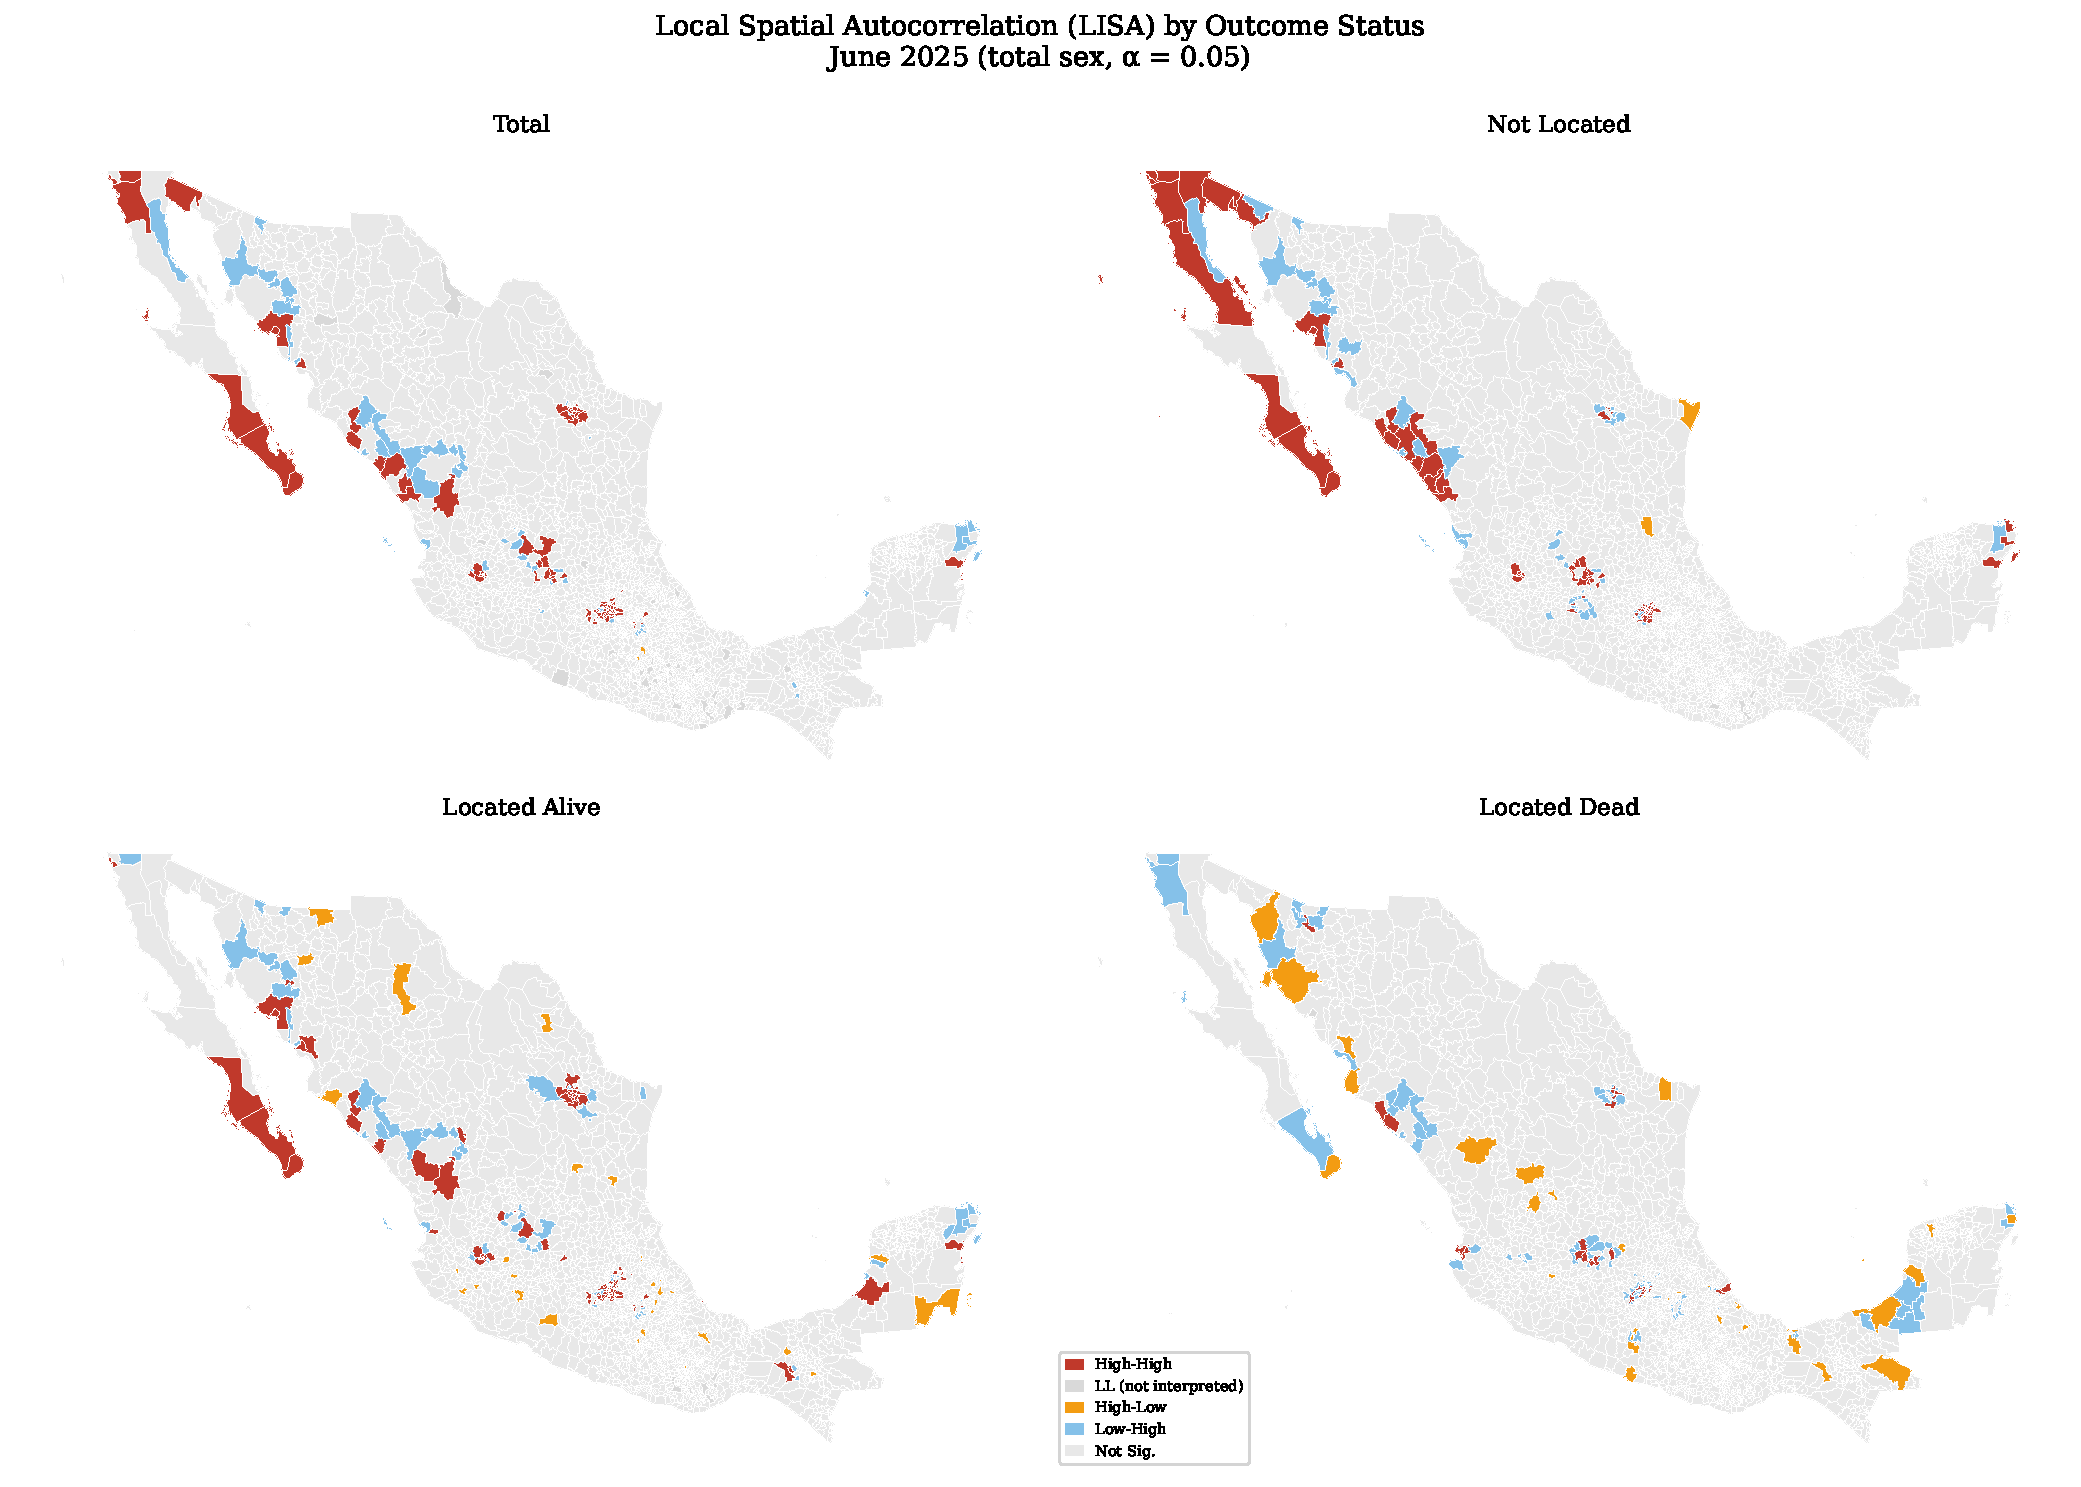
\includegraphics[width=\textwidth]{figures/fig4_lisa_maps_latest.pdf}
  \caption{LISA cluster maps by outcome status, \referencemonth{}.
           Red = High-High, grey = Low-Low (not interpreted; see Section~\ref{sec:lisa}),
           orange = High-Low, light blue = Low-High, white = Not Significant.
           Projection: EPSG:6372.}
  \label{fig:lisa_latest}
\end{figure}

\subsubsection{Non-Interchangeability: The Jaccard Evidence}

The paper's headline result is the quantitative demonstration that outcome statuses produce non-interchangeable spatial cluster geographies.
Table~\ref{tab:crosstab} reports pairwise Jaccard similarity coefficients (intersection over union of HH municipality sets) for \referencemonth{}.

\begin{tabular}{lrrrr}
  \toprule
  \textbf{} & \textbf{Total} & \textbf{Not Loc.} & \textbf{Located\,Alive} & \textbf{Located\,Dead} \\
  \midrule
  Total & \textbf{79} & 56 & 70 & 14 \\
  Not Loc. & 56 & \textbf{68} & 49 & 8 \\
  Located\,Alive & 70 & 49 & \textbf{91} & 12 \\
  Located\,Dead & 14 & 8 & 12 & \textbf{26} \\
  \bottomrule
  \multicolumn{5}{l}{\footnotesize Diagonal = total HH municipalities per status. Off-diagonal = pairwise intersection count.} \\
  \multicolumn{5}{l}{\footnotesize Reference period: June 2025. All counts use total sex LISA ($\alpha=0.05$).} \\
\end{tabular}

The Jaccard coefficients involving Located Dead are strikingly low: NL$\leftrightarrow$LD = 0.143 and LA$\leftrightarrow$LD = 0.151.
Only 14--15\% of the municipalities identified as hotspots for lethal outcomes overlap with hotspots for either Not Located or Located Alive cases.
The NL$\leftrightarrow$LA pair shows moderate overlap (0.381), suggesting some shared geography between active disappearances and recoveries.
The Total$\leftrightarrow$LA pair is highest (0.674), as expected given that Located Alive cases numerically dominate the Total series.

These results are stable across reference periods.
The Spearman rank correlation of local Moran's $I_i$ values between June 2024 and June 2025 ranges from 0.249 (Located Dead, total sex) to 0.607 (Total, total sex), confirming temporal stability in the underlying spatial structure (Appendix~\ref{app:robustness}).
The Jaccard pattern is also consistent across earlier cross-sections: in \bookendstart{}, NL$\leftrightarrow$LD Jaccard was 0.103 and LA$\leftrightarrow$LD was 0.000 (no overlap whatsoever between Located Alive and Located Dead hotspots).

% ==============================================================================
% Section 4.4: Temporal Dynamics (RQ3)
% ==============================================================================
\subsection{Temporal Dynamics (RQ3)}
\label{sec:temporal}

Having established that the four statuses cluster in different places, we now examine how those spatial patterns have evolved since 2015.
Table~\ref{tab:slopes} reports OLS trend slopes (Newey-West HAC standard errors, bandwidth = 12) for HH municipality counts by region and status.
Three regional narratives deserve attention.

\begin{tabular}{lrrrr}
  \toprule
  \textbf{Region} & \textbf{Total} & \textbf{Not Located} & \textbf{Located Alive} & \textbf{Located Dead} \\
  \midrule
  Norte & +0.55*** & +0.19 & +0.95*** & +0.54*** \\
  Norte-Occidente & +0.60*** & +0.44*** & +0.68*** & +0.06 \\
  Centro-Norte & -0.73*** & -0.50*** & -0.03 & +0.01 \\
  Centro & +2.82*** & +4.17*** & +3.13*** & +1.02*** \\
  Sur & +0.05 & +0.29*** & +0.12 & +0.03 \\
  Bajío & -0.99*** & +0.17 & -0.41* & +0.22* \\
  \bottomrule
  \multicolumn{5}{l}{\footnotesize OLS slope (municipalities per year $= $ slope $\times 12$), 132 monthly observations.} \\
  \multicolumn{5}{l}{\footnotesize $^{***}p<0.001$, $^{**}p<0.01$, $^{*}p<0.05$. Sign: positive $=$ growing hotspot region.} \\
\end{tabular}

\subsubsection{The Centro Expansion}

Centro emerges as the fastest-growing hotspot region across all four statuses---a finding that was invisible to prior annual analyses focused on the Norte--Baj\'{i}o axis.
Not Located HH municipalities in Centro grew at $+4.96$ municipalities per year ($p < 0.001$), the largest slope in the entire matrix.
Total ($+3.43$, $p < 0.001$), Located Alive ($+3.63$, $p < 0.001$), and Located Dead ($+1.26$, $p < 0.001$) all show significant positive trends.

Figure~\ref{fig:hh_trend} illustrates the divergent trajectories of Centro, Norte, and Baj\'{i}o.
The Centro expansion is visible as a steep upward trajectory beginning around 2019 for Not Located and accelerating through 2025.
This finding requires careful interpretation.
Two non-exclusive hypotheses may explain the pattern: (i) a real increase in disappearances in the metropolitan corridor spanning Estado de M\'{e}xico, CDMX, Puebla, Morelos, and Hidalgo---possibly reflecting urbanization of organized criminal violence; or (ii) a reporting artefact, whereby urban areas with more prosecutors, civil society organizations, and media attention register a higher proportion of disappearances even if underlying incidence did not increase as sharply.
We cannot distinguish between these hypotheses with RNPDNO data alone.

\begin{figure}[htbp]
  \centering
  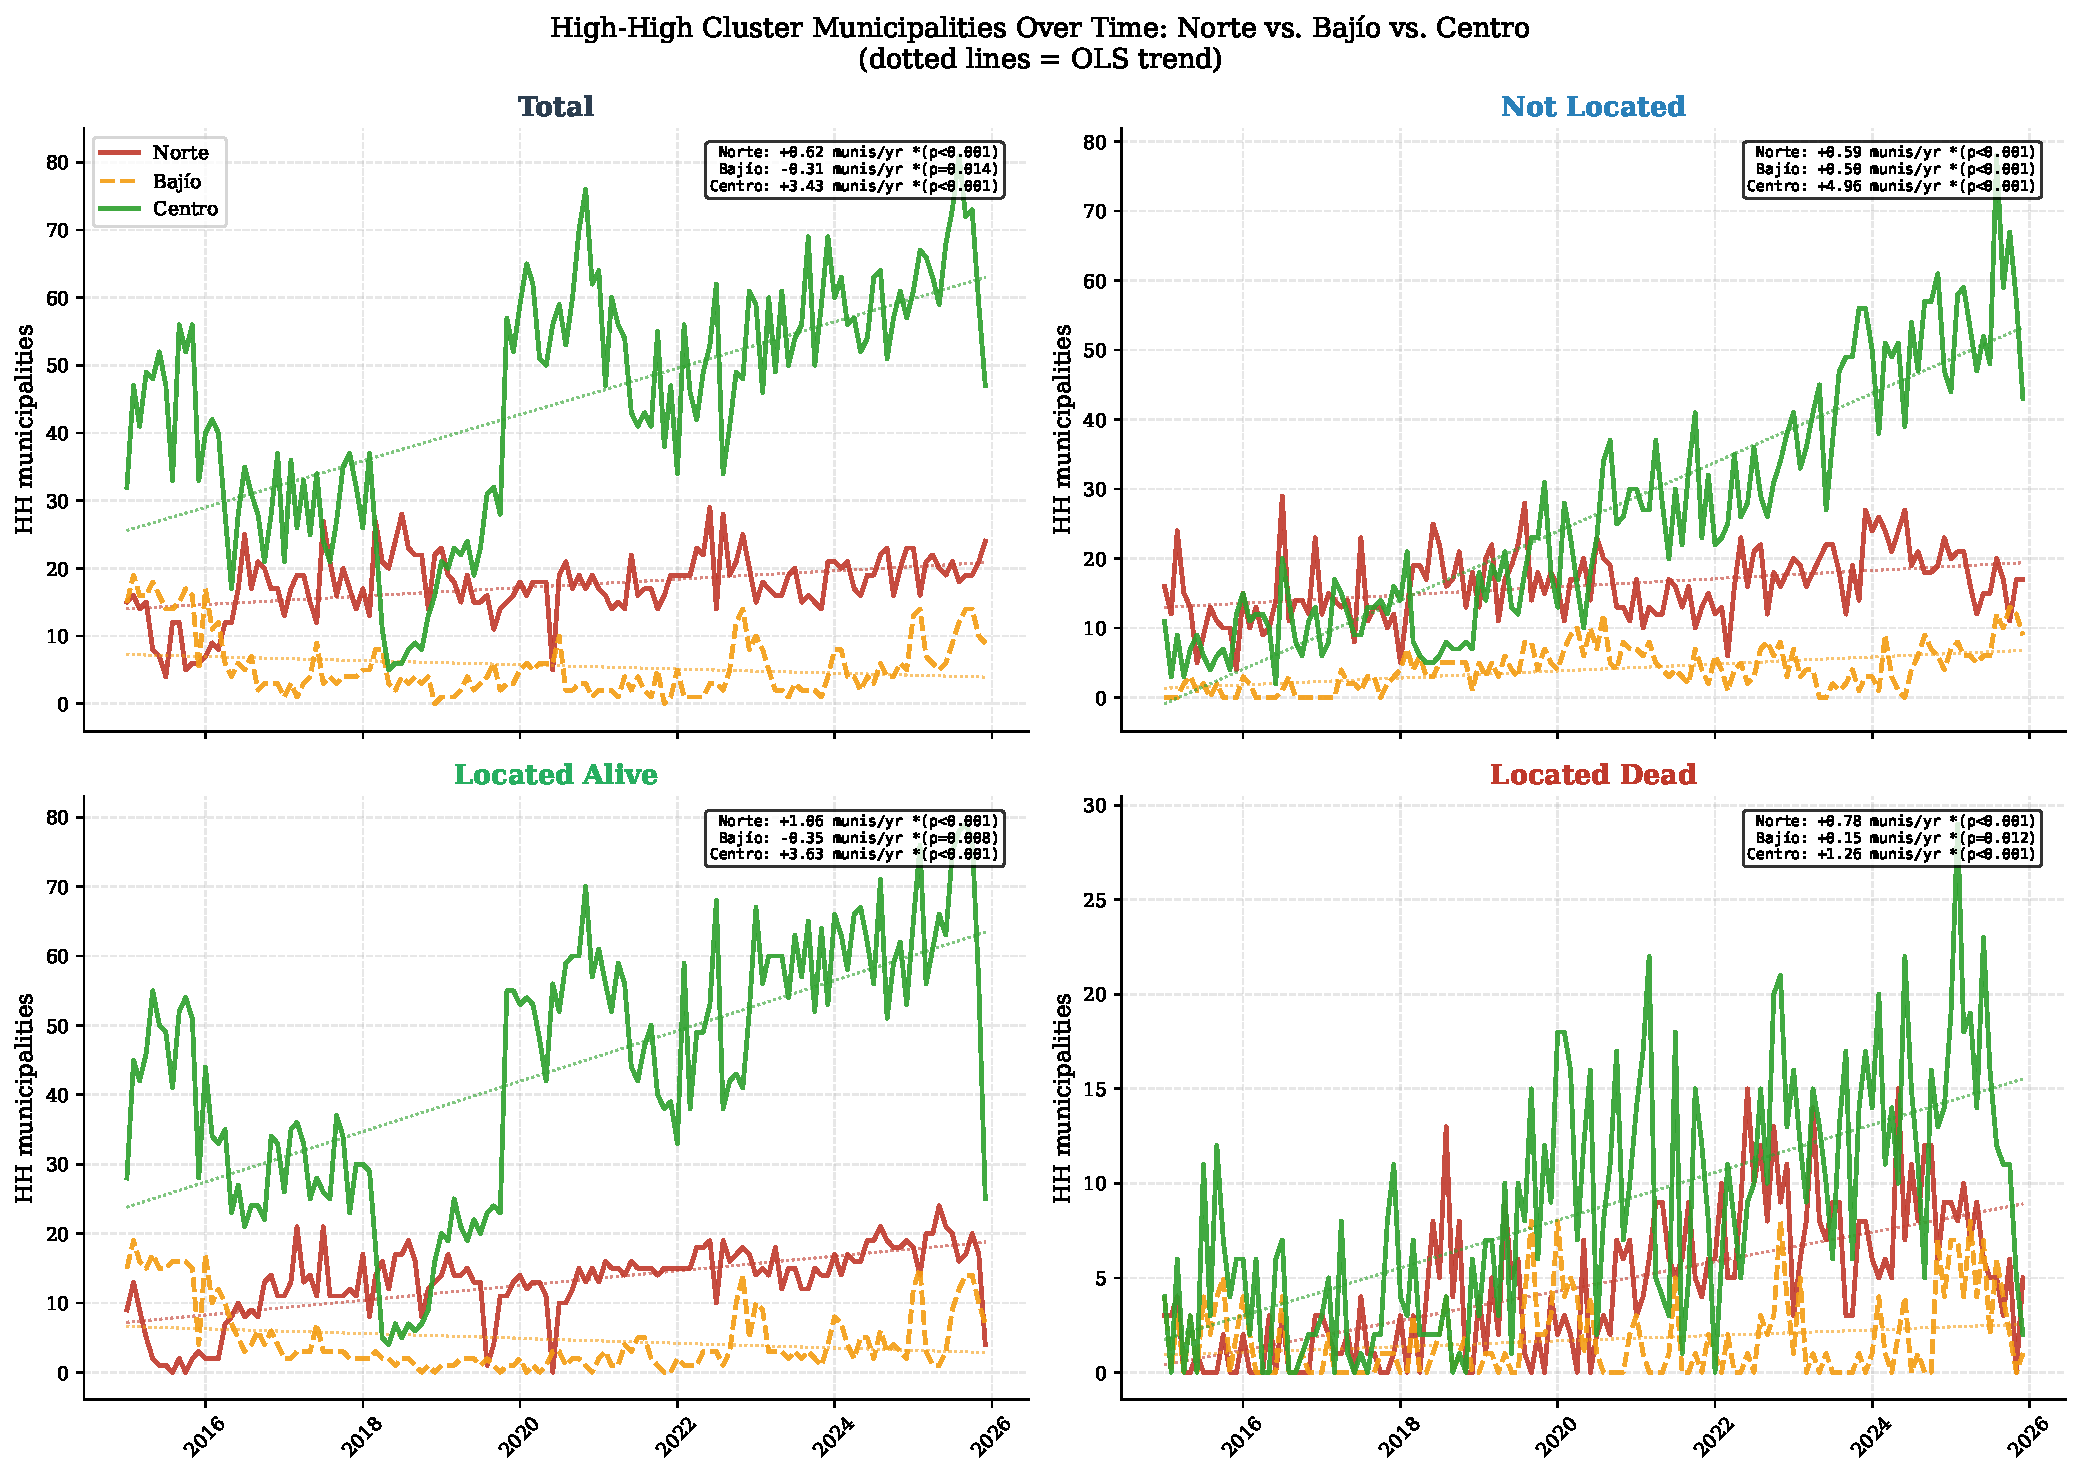
\includegraphics[width=\textwidth]{figures/fig5_hh_trend_norte_bajio.pdf}
  \caption{Monthly count of HH cluster municipalities in Norte (blue), Baj\'{i}o (orange), and Centro (green) by outcome status, \studyperiod{}.
           Dashed lines indicate OLS trends.
           Slopes (municipalities/year) annotated with Newey-West significance.}
  \label{fig:hh_trend}
\end{figure}

\subsubsection{The Norte Consolidation}

Norte shows consistent positive growth in HH municipalities across all four statuses: Total $+0.62^{*}$, Not Located $+0.59^{**}$, Located Alive $+1.06^{***}$, and Located Dead $+0.78^{***}$.
This multi-status consolidation suggests an entrenched organized crime presence---people are going missing, being found alive, \emph{and} being found dead at increasing rates in the same region.
The simultaneous growth of Located Alive and Located Dead hotspots in Norte may reflect a combination of high disappearance incidence and relatively developed forensic and search infrastructure: bodies and living persons are recovered because institutional capacity exists to register them, even as the underlying crisis deepens.

\subsubsection{The Baj\'{i}o Hypothesis: Rejected}

The earlier annual pipeline and existing literature \citep{cadena_garrocho_2019} suggested a ``rising Baj\'{i}o'' pattern driven by cartel territorial expansion into the Guanajuato--Jalisco corridor.
The monthly analysis rejects this hypothesis for the aggregate measure: Baj\'{i}o Total slope is $-1.09$ municipalities per year ($p = 0.024$), indicating a \emph{declining} hotspot footprint.
Located Alive in Baj\'{i}o also shows a negative (though non-significant) slope ($-0.47$, $p = 0.410$).
Located Dead trends positive ($+0.22$) but is not statistically significant ($p = 0.317$).
Not Located is similarly non-significant ($+0.24$, $p = 0.531$).

The Baj\'{i}o finding illustrates a broader methodological point: aggregate analyses can mask compositional dynamics that only become visible with outcome disaggregation and monthly resolution.

\subsubsection{Bookend Comparison}

Figure~\ref{fig:lisa_comparison} compares LISA maps for \bookendstart{} and \referencemonth{} for Located Alive and Located Dead, visualizing the geographic shift over the study period.
The expansion of Located Alive HH clusters from a concentrated Norte-Centro nucleus in 2015 to a broader multi-regional pattern by 2025 is clearly visible.
Located Dead clusters remain sparse at both endpoints, though a new cluster in Guanajuato emerges by 2025.

\begin{figure}[htbp]
  \centering
  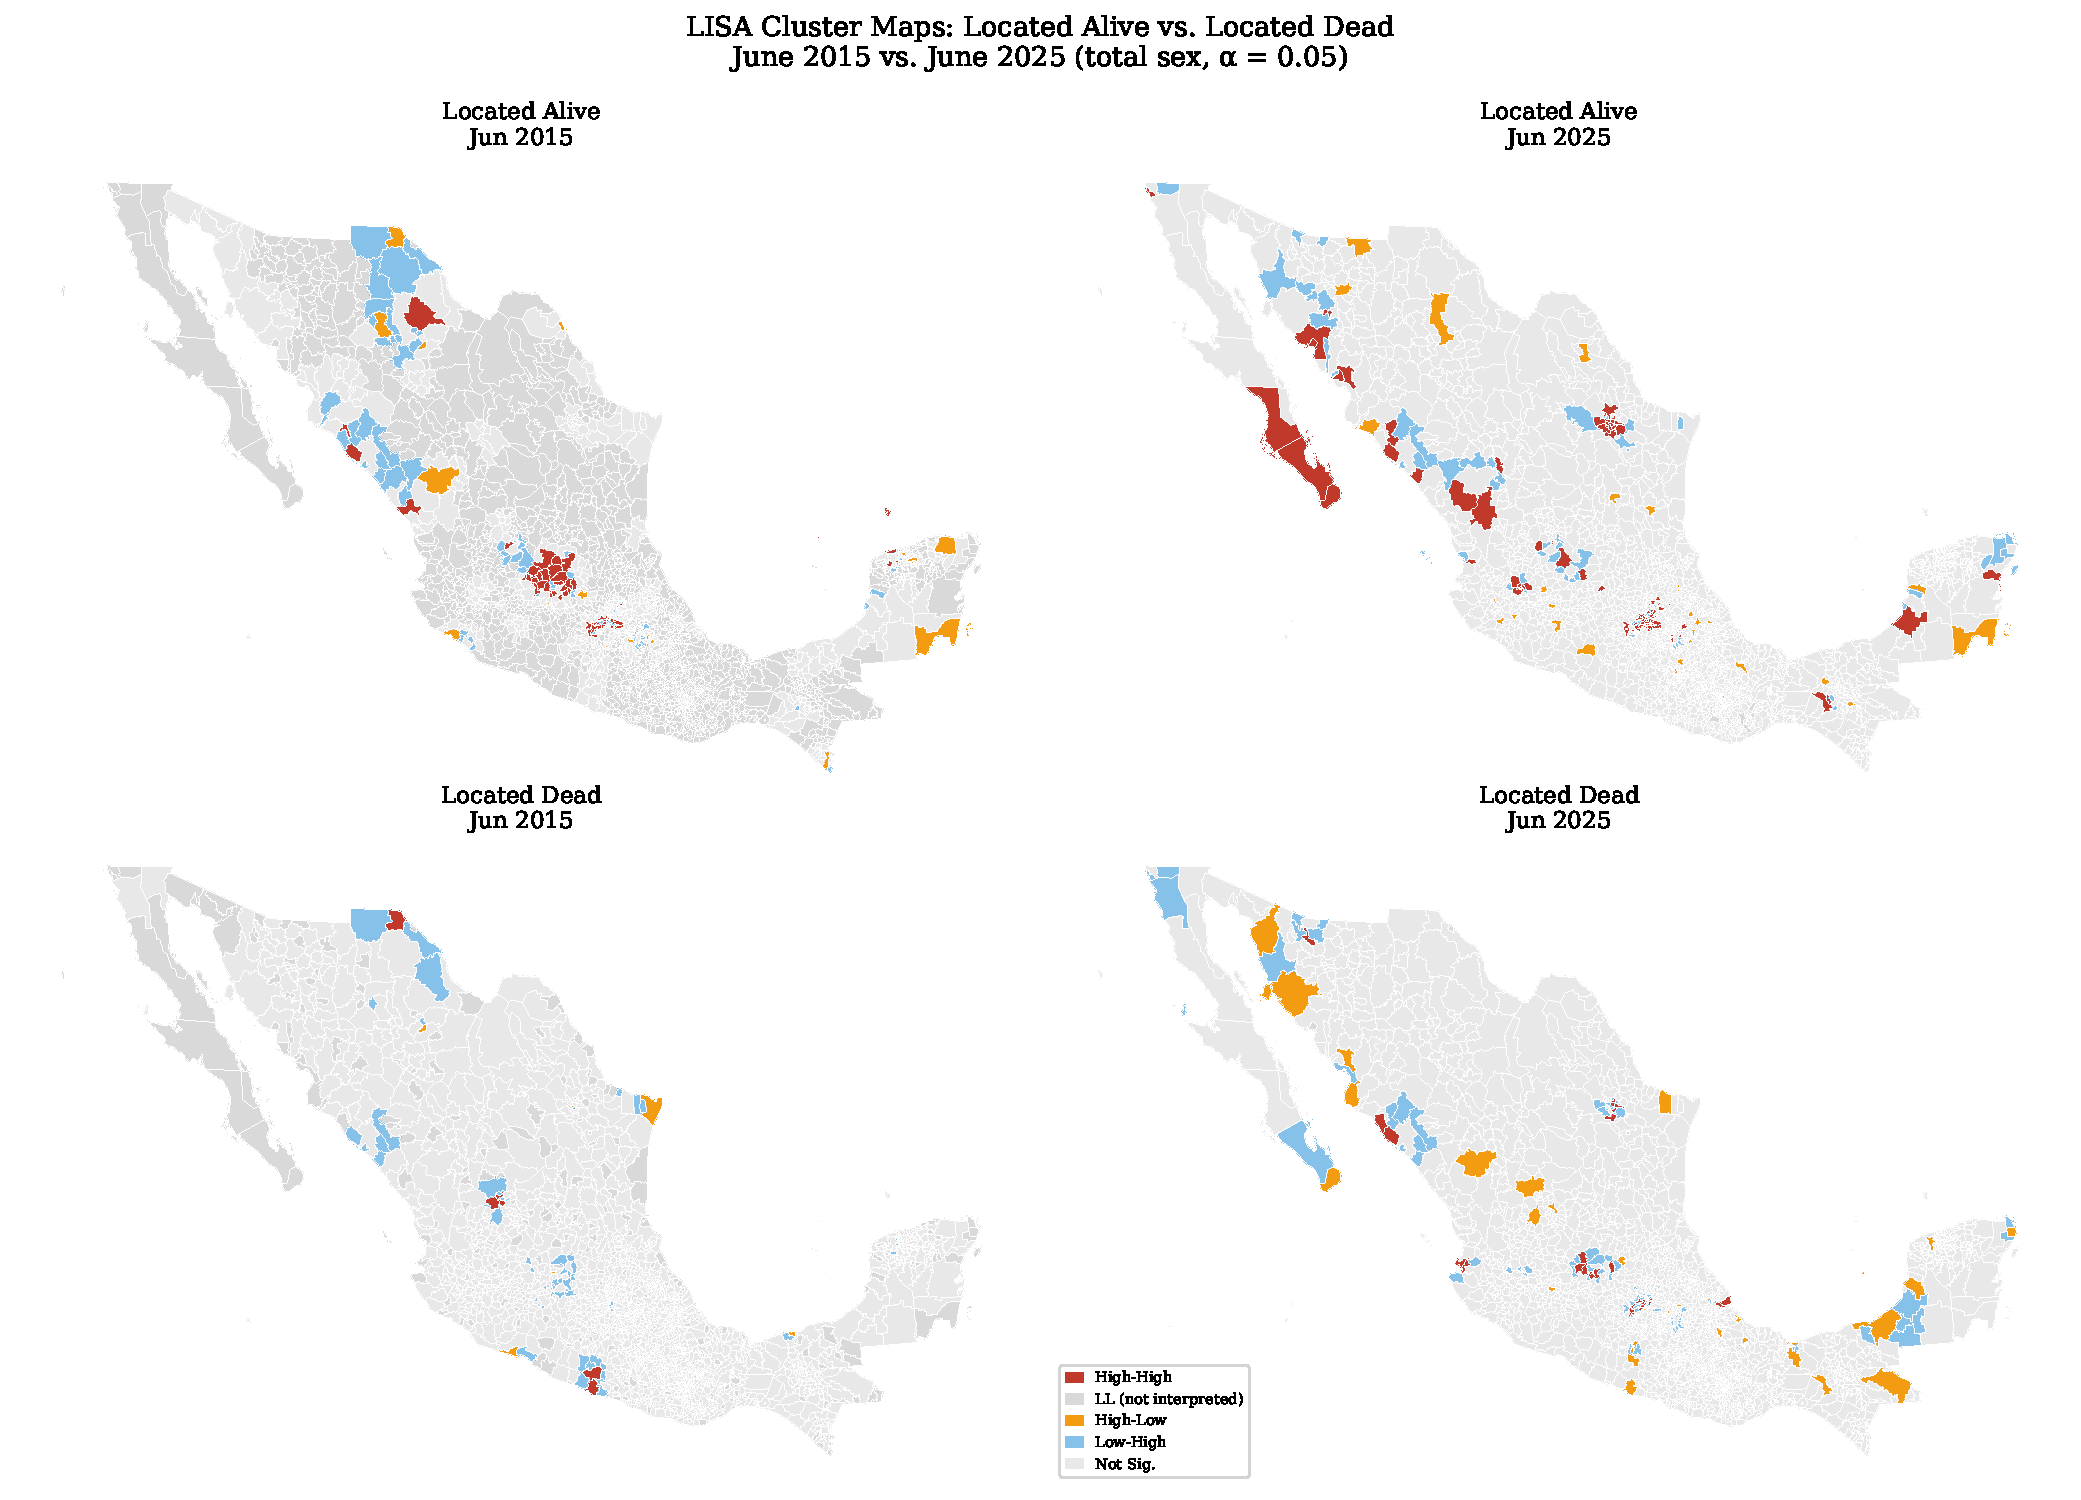
\includegraphics[width=\textwidth]{figures/fig6_lisa_maps_2015_vs_2025.pdf}
  \caption{LISA cluster maps for Located Alive (top) and Located Dead (bottom),
           \bookendstart{} (left) vs.\ \referencemonth{} (right).
           Projection: EPSG:6372.}
  \label{fig:lisa_comparison}
\end{figure}

Figure~\ref{fig:heatmap} provides a synoptic view of regional dynamics through a heatmap of HH municipality counts across 11 June snapshots (2015--2025) for all four statuses.
The chi-square tests for distributional change between \bookendstart{} and \referencemonth{} are significant for all statuses: Total ($\chi^2 = 9.5$, $p = 0.050$), Not Located ($\chi^2 = 16.5$, $p = 0.002$), Located Alive ($\chi^2 = 17.7$, $p = 0.001$), and Located Dead ($\chi^2 = 14.1$, $p = 0.007$).

\begin{figure}[htbp]
  \centering
  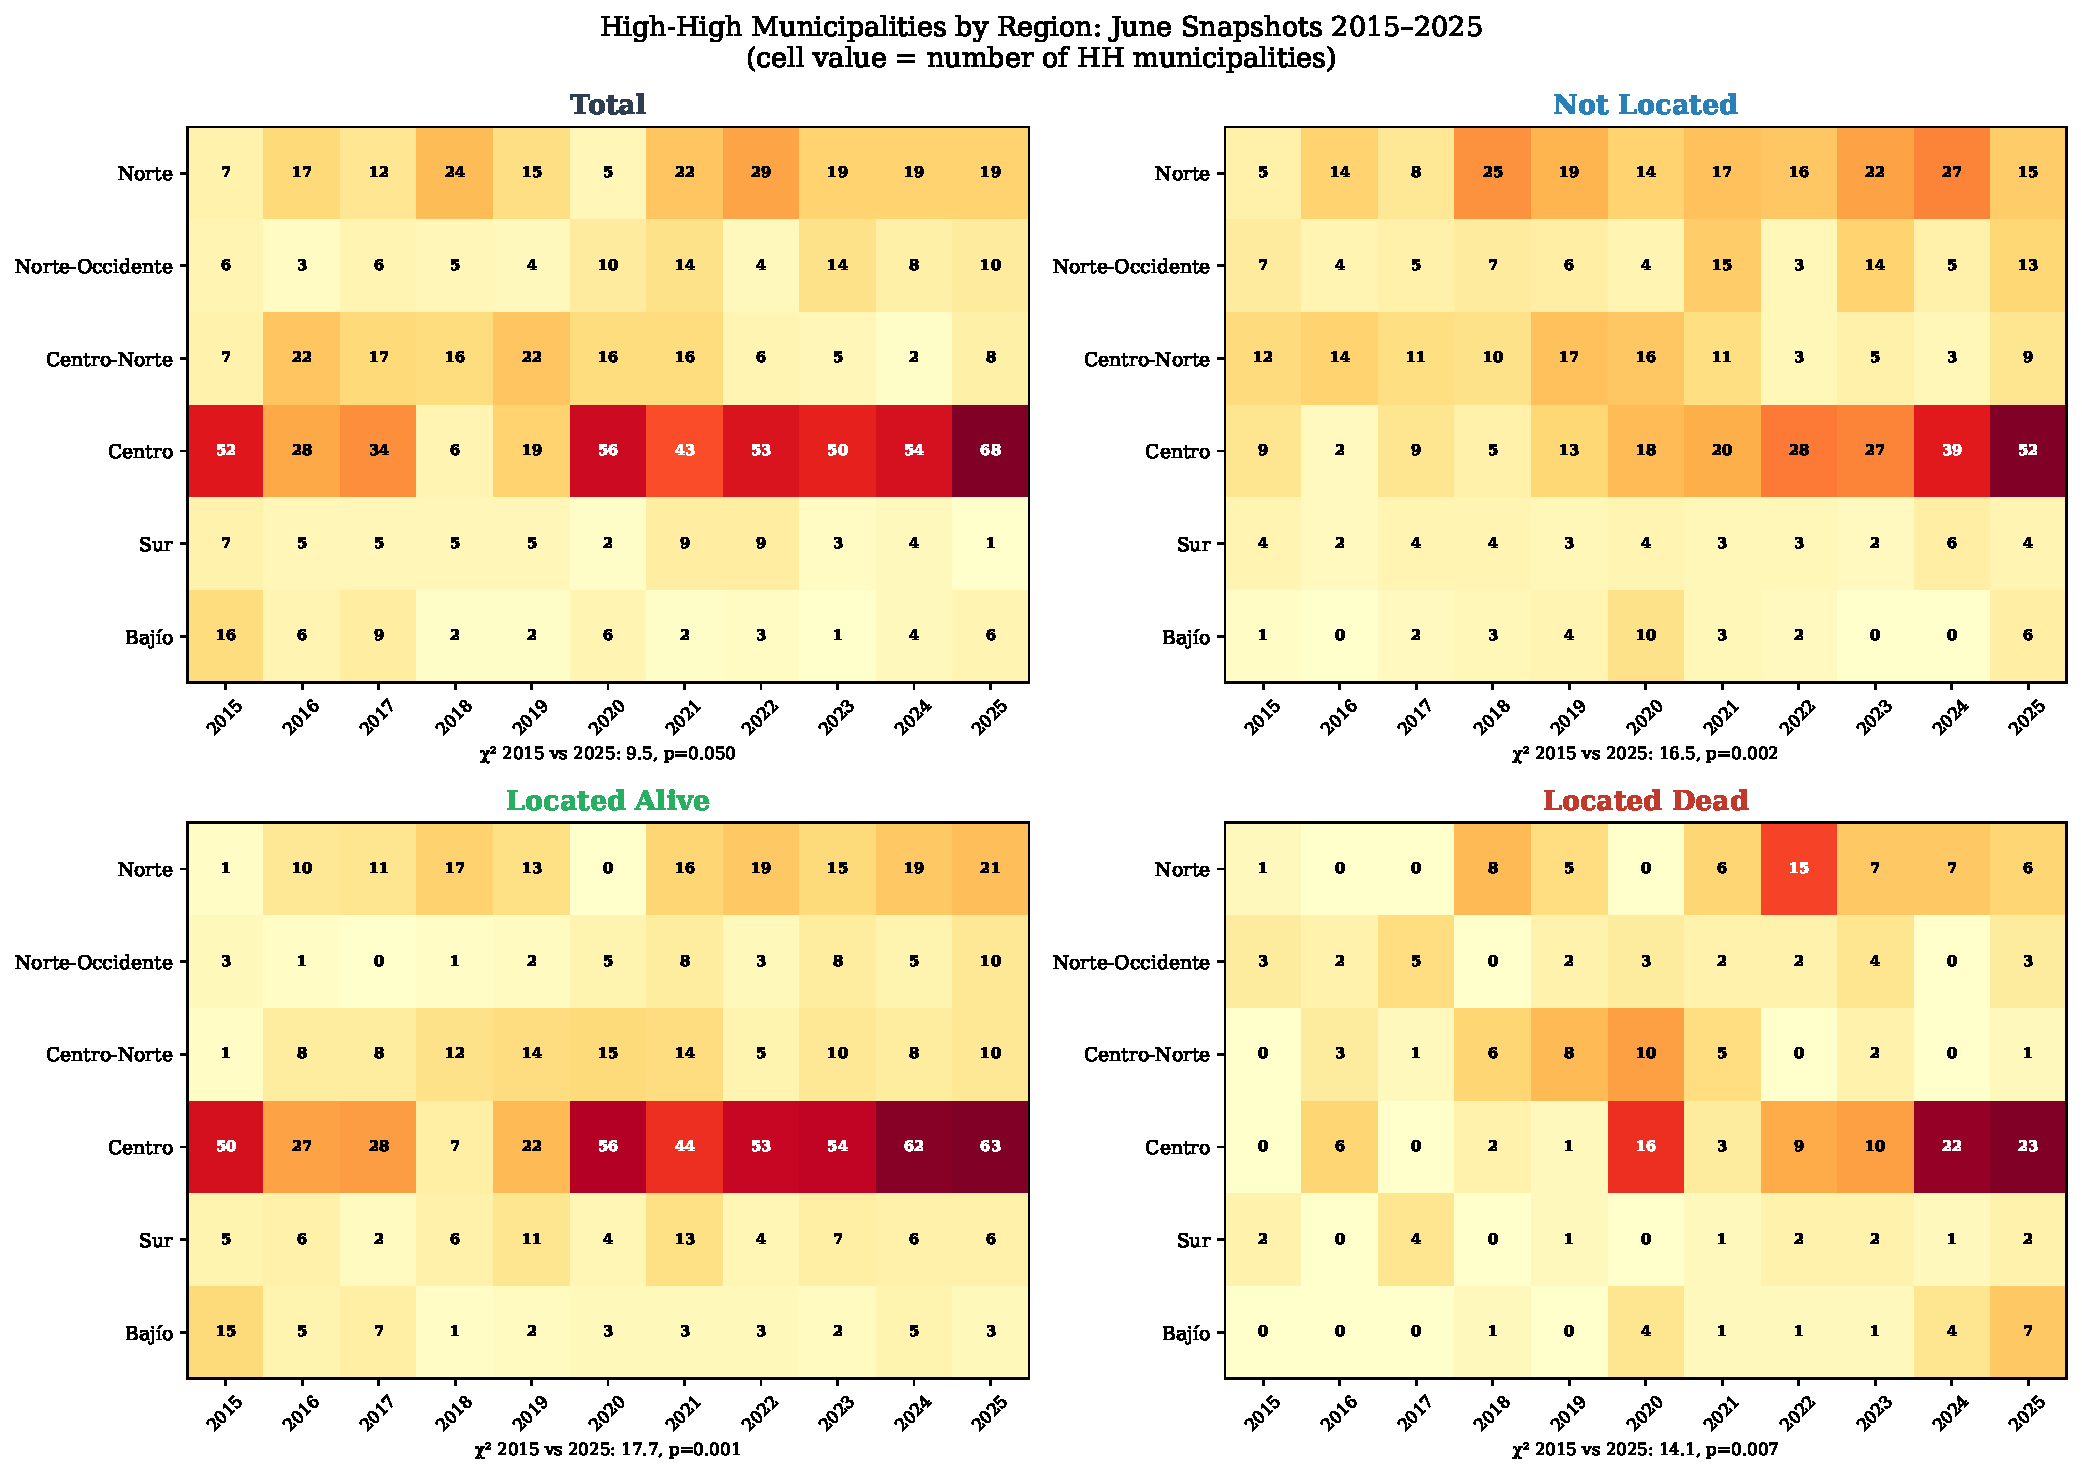
\includegraphics[width=\textwidth]{figures/fig8_regional_hh_heatmap.pdf}
  \caption{Regional HH heatmap: number of HH municipalities by region (rows) and June snapshot year (columns), four panels by outcome status.
           \bookendstart{} vs.\ \referencemonth{}.}
  \label{fig:heatmap}
\end{figure}

% ==============================================================================
% Section 4.5: Sex Disaggregation (RQ4)
% ==============================================================================
\subsection{Sex Disaggregation (RQ4)}
\label{sec:sex}

As documented in Section~\ref{sec:data}, the four outcome statuses differ substantially in their sex composition.
We now examine whether these aggregate differences translate into distinct spatial clustering patterns.

Figure~\ref{fig:sex_maps} compares male and female LISA maps for Not Located and Located Dead in \referencemonth{}.

\begin{figure}[htbp]
  \centering
  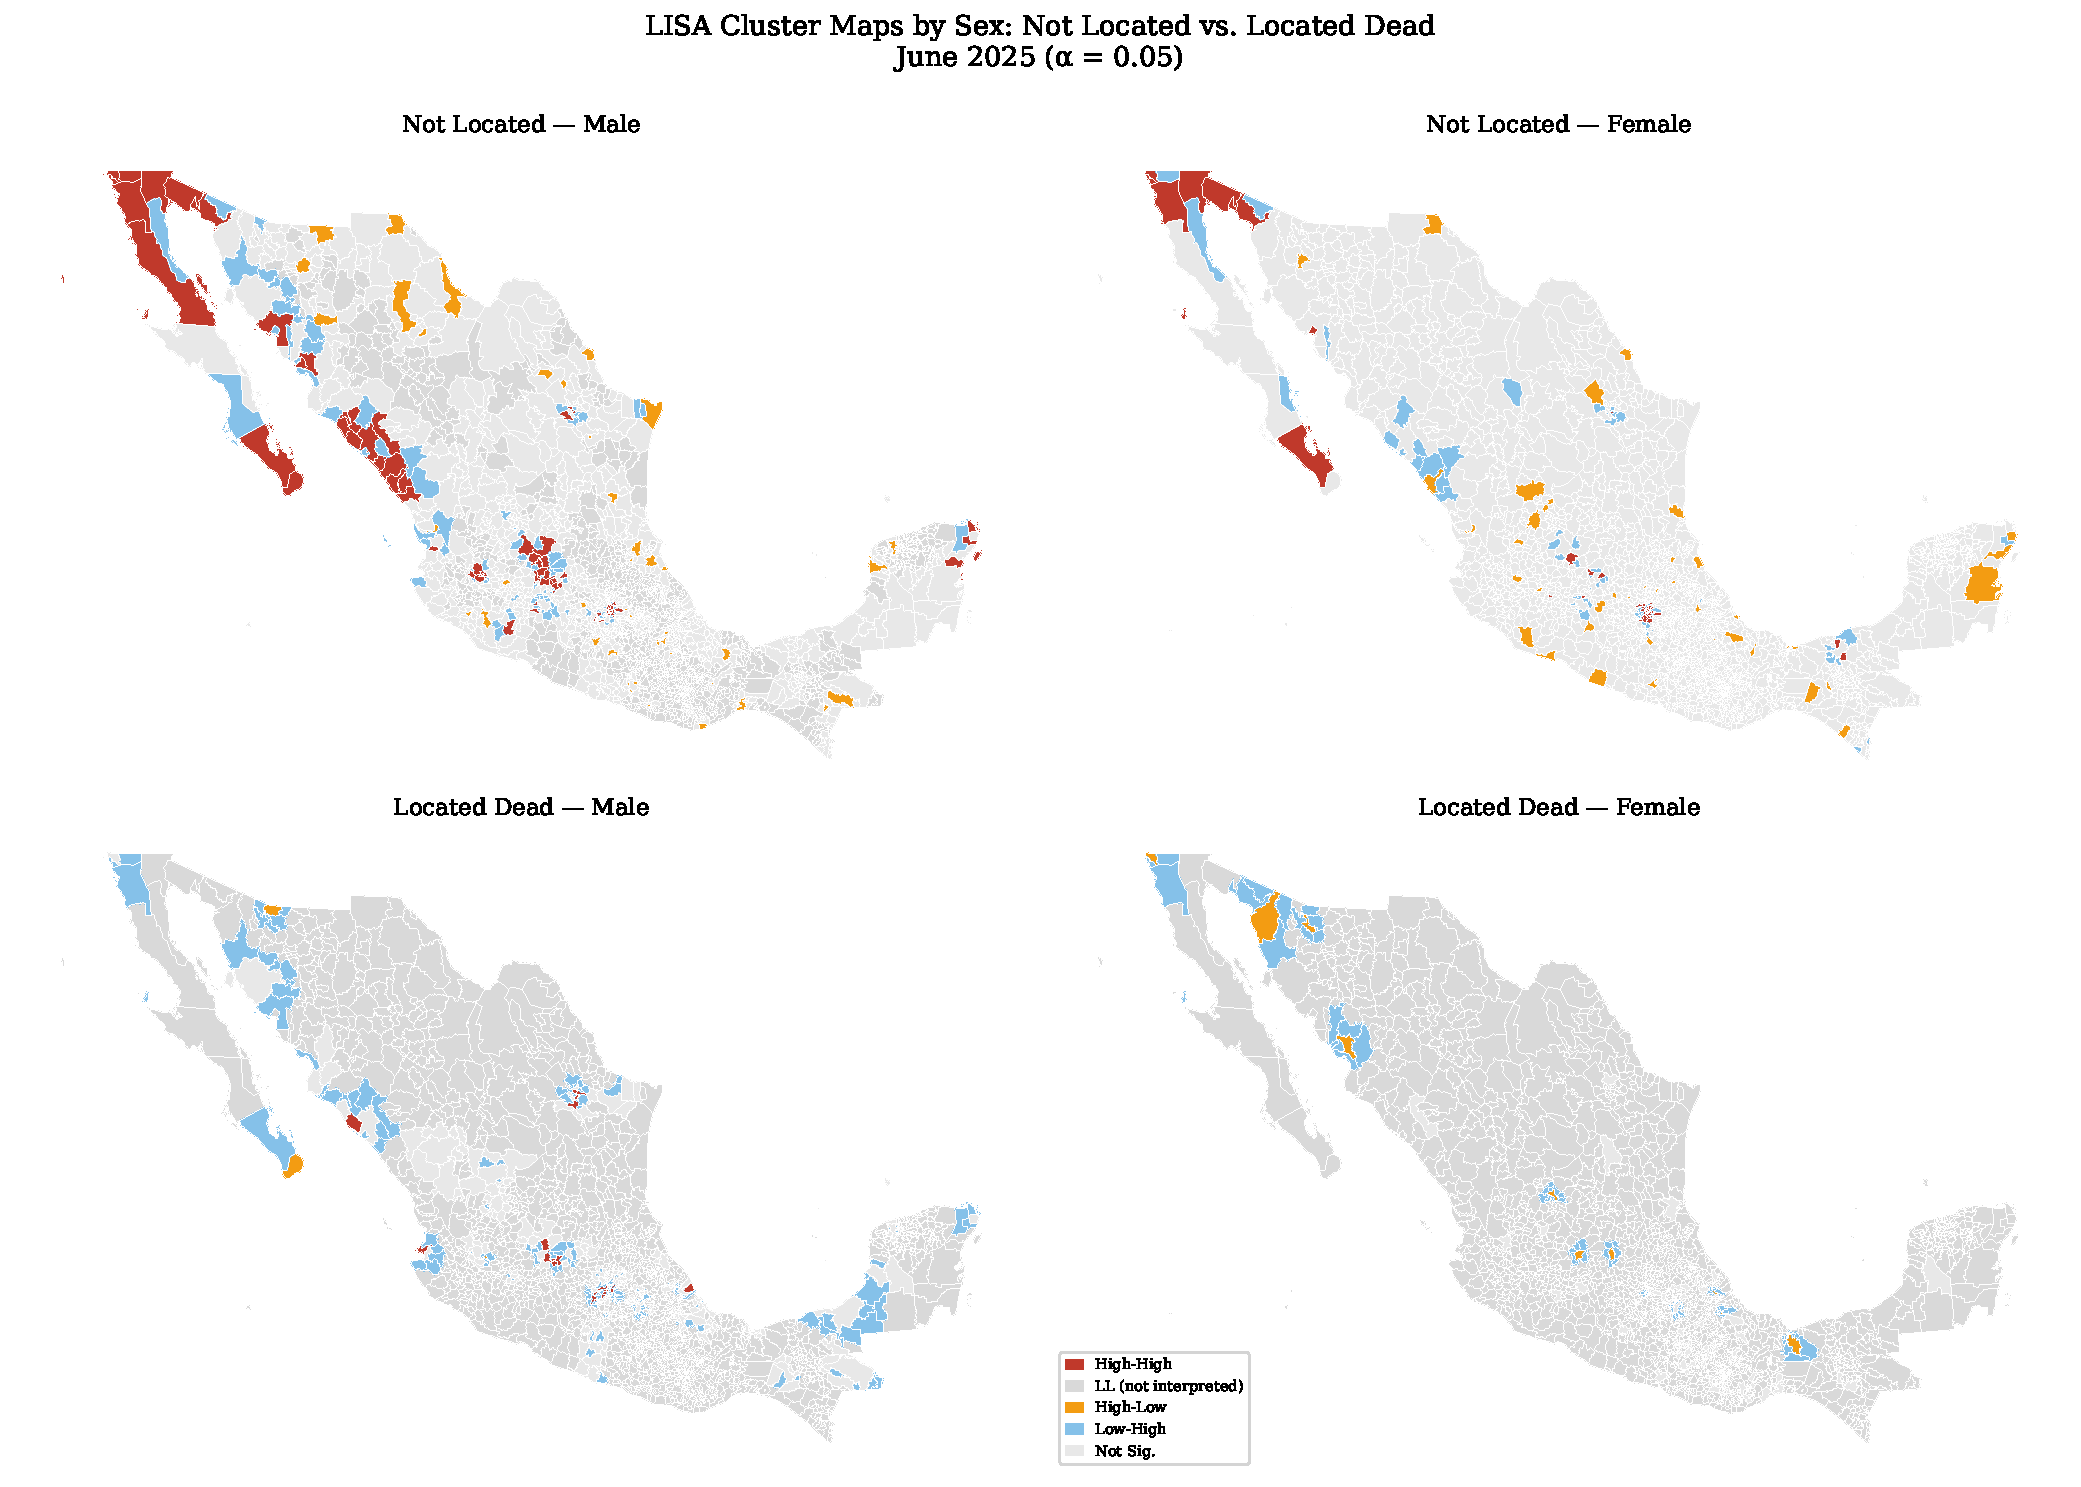
\includegraphics[width=\textwidth]{figures/fig7_sex_disaggregation_maps.pdf}
  \caption{LISA cluster maps by sex for Not Located (top) and Located Dead (bottom),
           \referencemonth{}.
           Left = male; right = female. Projection: EPSG:6372.}
  \label{fig:sex_maps}
\end{figure}

Table~\ref{tab:sex} quantifies the overlap between male and female HH classifications.

\begin{tabular}{lrrrrrr}
  \toprule
  \textbf{Status} & \textbf{Total HH} & \textbf{Male HH} & \textbf{Female HH} & \textbf{M $\cap$ F} & \textbf{M only} & \textbf{F only} \\
  \midrule
  Total & 80 & 84 & 73 & 55 & 29 & 18 \\
  Not Located & 71 & 66 & 40 & 23 & 43 & 17 \\
  Located Alive & 93 & 68 & 82 & 49 & 19 & 33 \\
  Located Dead & 17 & 15 & 0 & 0 & 15 & 0 \\
  \bottomrule
  \multicolumn{7}{l}{\footnotesize Reference period: June 2025. $\alpha=0.05$, Queen contiguity, 999 permutations.} \\
  \multicolumn{7}{l}{\footnotesize M $\cap$ F = municipalities HH under both male and female LISA. M/F only = sex-exclusive hotspots.} \\
\end{tabular}

For Total, 121 municipalities are classified as male HH and 99 as female HH, with 74 municipalities classified as HH for both sexes (Jaccard = 0.507).
Located Alive shows a similar pattern: 83 male HH, 90 female HH, and 58 shared (Jaccard = 0.504).
The moderate Jaccard values indicate that roughly half of the hotspot geography is shared, while the remainder is sex-specific.

Not Located exhibits greater divergence: 85 male HH versus 50 female HH, with only 28 shared municipalities (Jaccard = 0.262).
The lower female count reflects the male-dominated sex composition of Not Located cases (77.9\% male); fewer municipalities generate sufficient female-only counts to reach HH significance.
The low overlap suggests that the few municipalities with concentrated female Not Located cases are not the same municipalities driving male Not Located clustering.

Located Dead presents the starkest result: 27 male HH municipalities but \emph{zero} female HH municipalities (Jaccard = 0.000).
This is not a substantive finding about gendered victimization geography; it is a statistical power failure.
With a mean of 0.0065 female Located Dead cases per municipality-month and 99.4\% of cells recording zero, the LISA algorithm lacks sufficient spatial variation to detect any clusters.
Female Located Dead results should be excluded from policy interpretation.

% ==============================================================================
% Section 4.6: CED Alignment
% ==============================================================================
\subsection{CED Alignment}
\label{sec:ced}

In March 2026, the UN Committee on Enforced Disappearances (CED) issued its first-ever referral to the General Assembly under Article~34 of the Convention, finding that enforced disappearances in Mexico constitute crimes against humanity \citep{CED_MEX_art34_2026}.
The decision identifies ``multiple attacks at different moments and in different parts of the territory'' and names eight states as particular loci of concern.
Our LISA analysis provides the first national-scale quantitative evidence bearing on these geographic claims.

Figure~\ref{fig:ced_states} presents the HH dynamics for the eight CED-named states.

\begin{figure}[htbp]
  \centering
  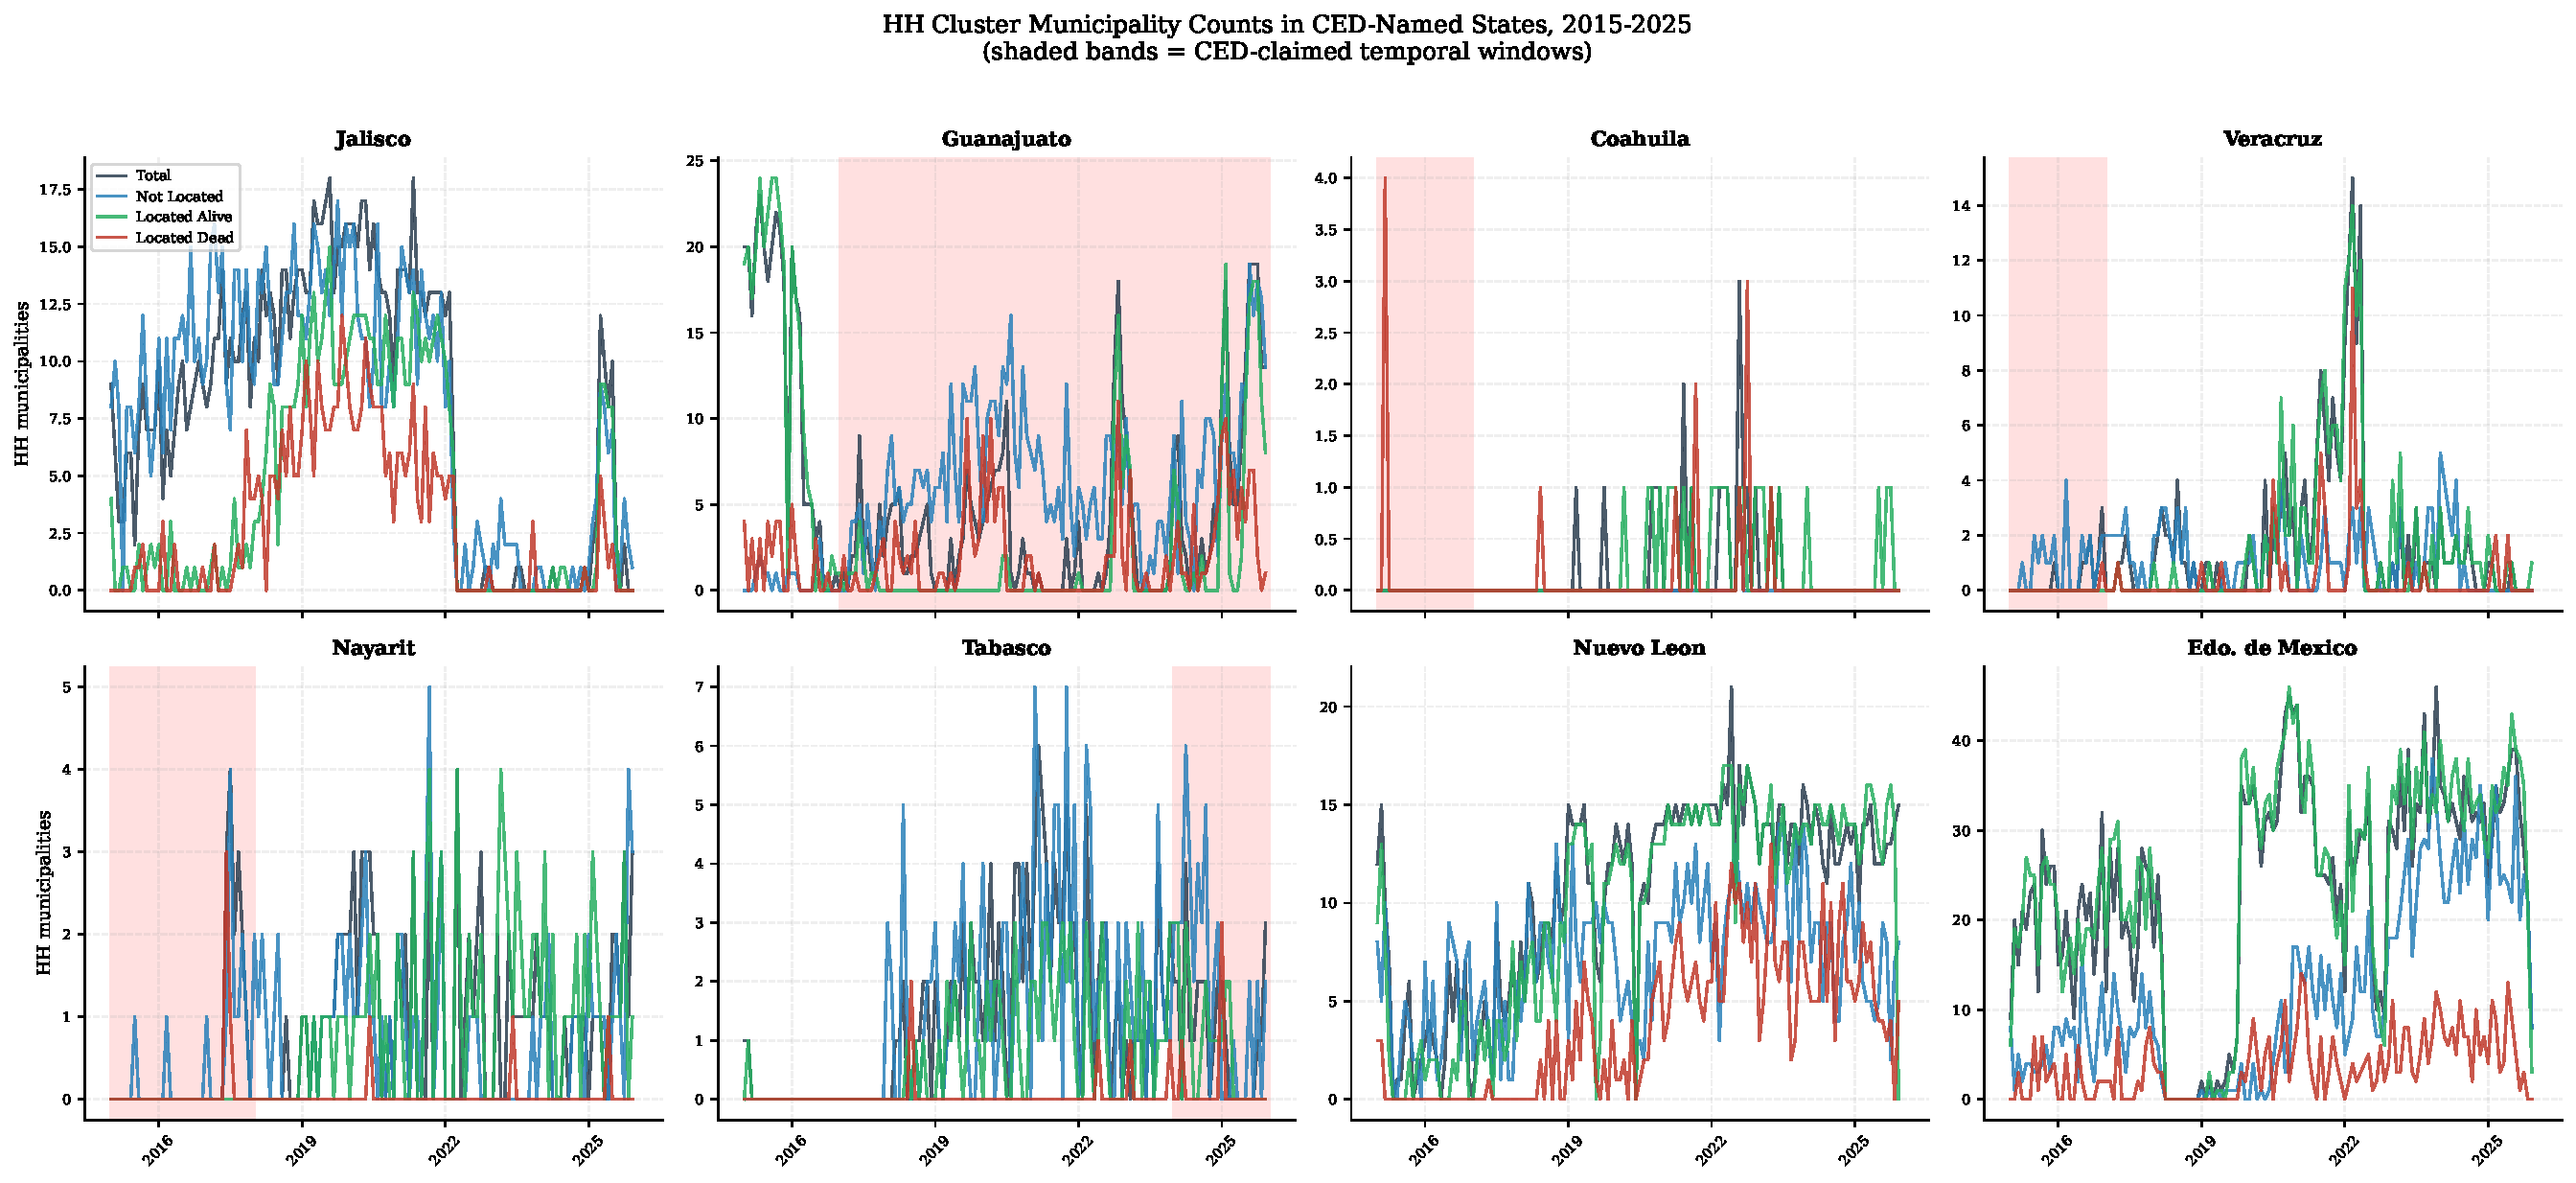
\includegraphics[width=\textwidth]{figures/fig9_ced_states.pdf}
  \caption{Monthly count of HH municipalities in eight CED-named states by outcome status, \studyperiod{}.
           Shaded bands indicate CED-referenced temporal windows.}
  \label{fig:ced_states}
\end{figure}

\textbf{Estado de M\'{e}xico} shows the strongest growth of any CED-named state: Not Located HH municipalities increased at $+2.36$ per year ($p < 0.001$), and Located Alive at $+1.81$ per year ($p < 0.001$).
The CED's temporal window (2015--2025) is fully aligned with the observed expansion.

\textbf{Nuevo Le\'{o}n} exhibits robust multi-status growth: Located Alive $+1.34$/yr ($p < 0.001$) and Located Dead $+0.80$/yr ($p < 0.001$).
HH peaks occur in 2022--2023, consistent with civil society reports of intensified organized criminal activity in the Monterrey metropolitan area.

\textbf{Guanajuato} presents a compositional shift.
Not Located HH municipalities are rising ($+0.75$/yr, $p < 0.001$), but Located Alive is declining ($-0.57$/yr, $p < 0.001$).
The CED's characterization of an ``eightfold increase since 2017'' aligns with the Not Located trajectory but not with the Located Alive decline---fewer people are being found alive even as more remain not located.

\textbf{Jalisco} shows declining HH municipalities across all statuses, with peaks around 2019.
This appears to contradict the CED's characterization of Jalisco as ``currently highest'' in disappearances; however, our HH metric captures spatial \emph{clustering}, not absolute volume.
A state may have high absolute counts but spatially diffuse registrations that do not produce significant local clusters.

\textbf{Coahuila, Veracruz, and Nayarit} show low or zero HH municipalities throughout most of the study period.
The CED's temporal claims for these states reference crisis periods (2009--2017) that largely predate or fall at the beginning of our study window, limiting our ability to capture the dynamics the CED describes.

\textbf{Tabasco} is flagged by the CED for an ``exponential increase 2024--2025'' with specific concern for girls and women.
Our sex-disaggregated analysis provides partial support: female Located Alive HH municipality-months (31) substantially exceed male (6) in 2023--2025, consistent with the CED's claim of gendered victimization.
For Not Located, however, the pattern is reversed (male 39 municipality-months vs.\ female 34), and overall HH counts in Tabasco remain low.

We emphasize three caveats.
First, we do not adjudicate state responsibility; our analysis is descriptive.
Second, the RNPDNO aggregates all disappearances, not only enforced disappearances---the government's position is that many registered cases reflect non-state-actor crimes.
Our spatial clusters capture the composite phenomenon regardless of perpetrator type.
Third, several CED-named states exhibit low HH counts not because disappearances are absent but because the RNPDNO may undercount registrations in states with weaker institutional infrastructure.


% ==============================================================================
% ==============================================================================
% Section 5: Discussion
% ==============================================================================
\section{Discussion}
\label{sec:discussion}

\subsection{Non-Interchangeability of Outcome Statuses}
\label{sec:disc_noninterchange}

The central finding of this paper is that the four outcome statuses are not spatially interchangeable.
Jaccard coefficients below 0.15 for all pairs involving Located Dead demonstrate that the municipalities where lethal outcomes concentrate are fundamentally different from the municipalities where active disappearances or living recoveries cluster.
Even the highest pairwise overlap---Total and Located Alive at 0.674---leaves one-third of hotspot municipalities unshared.

This result has a direct analogue in the spatial criminology literature.
\citet{andresen_2006} demonstrated that counts and rates of the same crime type produce different hotspot geographies, leading to different policy conclusions depending on which metric is used.
Our finding extends this logic: even holding the metric constant (raw counts), different \emph{outcome categories} of the same underlying phenomenon produce non-overlapping spatial clusters.
The implication is analogous to \citeauthor{braga_law_2017}'s (\citeyear{braga_law_2017}) observation that crime type disaggregation matters for concentration analysis---here, outcome status disaggregation matters for disappearance analysis.

For policy, the non-interchangeability result means that forensic search teams---which should be deployed where bodies are found (Located Dead geography)---and prevention or active search programs---which should target areas of concentrated unresolved cases (Not Located geography)---cannot use the same geographic prioritization.
Treating disappearances as a single metric produces a composite map dominated by Located Alive cases (which account for 60\% of registrations), potentially directing resources away from the distinct municipalities where the most severe outcomes concentrate.

\subsection{Regional Dynamics}
\label{sec:disc_regional}

\subsubsection{Centro: Real Expansion or Reporting Artefact?}

The Centro region's emergence as the fastest-growing HH cluster---with Not Located slopes exceeding $+4.96$ municipalities per year---is the most surprising empirical finding of this study.
Prior literature on Mexico's disappearance crisis has focused almost exclusively on the Norte--Baj\'{i}o axis, where cartel territorial competition is well documented \citep{cadena_garrocho_2019, rios_2013}.
The Centro expansion went undetected in annual analyses because it began gradually around 2019 and accelerated through 2024--2025, a trajectory that requires monthly resolution to identify.

Two competing hypotheses may explain this pattern, and we cannot distinguish between them with the available data.
The first is a real increase in disappearances in the metropolitan corridor spanning Estado de M\'{e}xico, CDMX, Puebla, Morelos, and Hidalgo---potentially reflecting the urbanization of organized criminal violence as trafficking routes shift toward the capital region.
The second is a reporting artefact: urban areas with stronger prosecutorial capacity, more active civil society organizations, and greater media attention may register a higher proportion of cases even if underlying incidence did not increase as sharply.
The RNPDNO records registrations, not verified events.
Disentangling these hypotheses requires external covariates (prosecutorial capacity indices, media attention proxies) and is the subject of planned econometric work.

\subsubsection{Norte: Multi-Status Consolidation}

Norte's consistent positive slopes across all four statuses suggest an entrenched disappearance hotspot that is simultaneously deepening and revealing its outcomes.
The coexistence of growing Located Alive and Located Dead HH clusters may reflect a combination of high organized crime incidence and relatively developed forensic and search infrastructure in states such as Tamaulipas and Nuevo Le\'{o}n.
This interpretation---high violence \emph{and} institutional capacity---is a hypothesis; it could alternatively reflect that Norte's crisis has simply reached a scale at which all outcome categories produce detectable spatial clustering.

\subsubsection{Baj\'{i}o: Hypothesis Rejected}

The ``rising Baj\'{i}o'' hypothesis, suggested by \citet{cadena_garrocho_2019}'s 2006--2017 analysis and attributed to cartel route reorganization through the Guanajuato--Jalisco corridor, is rejected by our monthly data.
Baj\'{i}o Total HH municipalities declined at $-1.09$ per year ($p = 0.024$).
The non-significant Located Dead slope ($+0.22$, $p = 0.317$) prevents us from claiming a lethality increase.
If anything, the Baj\'{i}o pattern suggests a contracting hotspot footprint---though this could reflect displacement to adjacent regions rather than genuine improvement.

\subsection{CED Alignment}
\label{sec:disc_ced}

Our analysis provides the first national-scale quantitative evidence supporting the CED's characterization of enforced disappearances as involving ``multiple attacks at different moments and in different parts of the territory'' \citep{CED_MEX_art34_2026}.
The LISA results show HH clusters emerging, expanding, and shifting across states over \nmonths{} months---a pattern consistent with the CED's temporal and geographic narrative.

Three important qualifications apply.
First, the RNPDNO aggregates all disappearances regardless of perpetrator type; our spatial clusters capture the composite phenomenon, not enforced disappearances specifically.
The Mexican government has argued that many registered cases reflect private-actor violence, not state involvement \citep{CED_MEX_visit_2022}.
Our analysis is agnostic to this distinction.
Second, several CED-named states (Coahuila, Veracruz, Nayarit) show low or zero HH municipalities, which may reflect underreporting rather than absence of crisis.
Third, the discrepancy between our Jalisco finding (declining HH) and the CED's characterization (``currently highest'') highlights the difference between absolute volume and spatial clustering: a state may report the most disappearances nationally while those cases are too spatially diffuse to produce significant local clusters.

\subsection{Sex Patterns}
\label{sec:disc_sex}

The Located Alive near-parity result (49.4\% male, 50.5\% female) is puzzling in light of the male-dominated profile of Not Located cases (77.9\% male).
Women who disappear appear to be found alive at a rate disproportionate to their share of active disappearances.
Two possible mechanisms warrant investigation: (i) gender-specific disappearance types with different recovery profiles (e.g., domestic violence or trafficking cases involving women may have higher resolution rates); or (ii) differential registration practices (women's recoveries may be recorded more systematically due to advocacy pressure).
The spatial divergence in Not Located male vs.\ female HH (Jaccard = 0.262) suggests that these are not simply different counts in the same places but geographically distinct phenomena.

The female Located Dead power failure (zero HH municipalities) underscores a general limitation of spatial analysis applied to rare events: with mean counts near zero, no spatial method can detect meaningful patterns.

\subsection{Limitations}
\label{sec:limitations}

\begin{enumerate}
  \item \textbf{Raw counts without population normalization.}
        Concentration in large, high-population municipalities may partly reflect population size rather than elevated risk.
        A population-normalized companion analysis is forthcoming \citep[cf.][]{andresen_2006}.

  \item \textbf{Ecological fallacy.}
        Municipal-level analysis cannot support individual-level inferences about victimization risk or perpetrator behavior.

  \item \textbf{Zero-infilling assumption.}
        Municipality-months absent from the RNPDNO are treated as zero cases.
        If absences reflect reporting failure rather than true zeros, concentration metrics are underestimated in under-reporting municipalities, and the true geographic spread of disappearances is broader than our estimates suggest.

  \item \textbf{Spatial weights specification.}
        Queen contiguity may not capture functional connectivity such as road networks, cartel territorial boundaries, or institutional jurisdictions.
        Sensitivity to alternative weight matrices (k-nearest neighbors, distance-based) is left for future work.

  \item \textbf{Descriptive design.}
        This analysis documents spatial patterns; it does not identify causal mechanisms.
        All regional narratives are hypotheses requiring econometric testing.

  \item \textbf{Potential underreporting.}
        The RNPDNO relies on official registration.
        Disappearances in municipalities with weak state presence, high impunity, or low civil society activity may be systematically underreported, biasing hotspot maps toward high-capacity jurisdictions \citep{guercke_2021}.

  \item \textbf{Female Located Dead statistical power.}
        With a mean of 0.0065 cases per municipality-month and 99.4\% zero cells, LISA results for female Located Dead are uninformative and should not guide policy.

  \item \textbf{No enforced/non-enforced distinction.}
        The RNPDNO does not distinguish enforced disappearances (state involvement) from disappearances by private actors.
        Our spatial clusters capture both.

  \item \textbf{End-of-period reporting lag.}
        November--December 2025 totals show Dec/Jul ratios of 0.46--0.72, indicating incomplete registration.
        June cross-sections mitigate this for snapshot analyses, but full-series trend estimates include these lagged months.
\end{enumerate}


% ==============================================================================
% ==============================================================================
% Section 6: Conclusion
% ==============================================================================
\section{Conclusion}
\label{sec:conclusion}

This paper presents the first national-scale, outcome-disaggregated, monthly spatial analysis of disappearances in Mexico.
Covering \nmunis{} municipalities over \nmonths{} months (\studyperiod{}), it examines four outcome statuses---Total, Not Located, Located Alive, and Located Dead---through \nLISAruns{} LISA runs.

Five empirical facts are established.
First, disappearance outcome statuses are spatially non-interchangeable.
Jaccard similarity between Located Dead and either Not Located (0.143) or Located Alive (0.151) hotspots confirms that lethal-outcome geography is fundamentally distinct from the geography of active disappearances or living recoveries.
Second, geographic concentration exceeds standard criminological benchmarks by a factor of two to three: 50\% of Not Located cases in \referencemonth{} concentrated in just 42 municipalities (1.7\% of \nmunis{}), compared to the 4--6\% benchmark posited by \citet{weisburd_2015}.
Third, Centro is the fastest-growing hotspot region, with Not Located HH municipalities expanding at $+4.96$ per year ($p < 0.001$)---a trajectory invisible to annual analyses.
Fourth, the ``rising Baj\'{i}o'' hypothesis is rejected: Baj\'{i}o Total HH municipalities declined at $-1.09$ per year ($p = 0.024$).
Fifth, the CED's characterization of spatially and temporally heterogeneous attacks across Mexican states finds empirical support in the LISA dynamics, though with important caveats for states with low HH counts.

The policy implication is direct: outcome-specific geographic targeting is necessary.
Forensic identification resources should follow Located Dead hotspot geography, currently concentrated in Guanajuato and scattered municipalities in Tamaulipas and Jalisco.
Active search and prevention resources should follow Not Located hotspot geography, dominated by the rapidly expanding Centro corridor.
These are different places.
A composite ``disappearance map'' conflating all statuses would direct resources to a Located Alive--dominated geography that obscures the distinct municipalities where the most severe outcomes concentrate.

Future work will address the limitations of raw-count analysis.
A companion paper will introduce population-normalized rates and evaluate whether the non-interchangeability result holds under dual-metric (count and rate) analysis.
A subsequent econometric panel study will incorporate external covariates---organized crime incidence, prosecutorial capacity, socioeconomic indicators---to move from spatial description to causal inference.


% ==============================================================================
\bibliographystyle{apalike}
\bibliography{references}

% ==============================================================================
% ==============================================================================
% Appendix
% ==============================================================================
\appendix

\section{Robustness Checks}
\label{app:robustness}

\subsection{Temporal Stability of Local Moran's I}

To assess the temporal stability of the spatial structure, we compute Spearman rank correlations of municipality-level local Moran's $I_i$ values between the June 2024 and June 2025 cross-sections for each status$\times$sex combination.
All correlations are statistically significant ($p < 0.001$).
Values range from 0.227 (Located Dead, male) to 0.607 (Total, total), indicating moderate to strong rank-order stability across the twelve-month interval.
Located Dead shows the weakest correlations (0.227--0.303), consistent with the greater volatility expected from sparse count data.

\begin{table}[htbp]
  \centering
  \caption{Spearman rank correlation of local Moran's $I_i$ between June 2024 and June 2025.}
  \label{tab:spearman}
  \begin{tabular}{llcc}
    \toprule
    Status & Sex & Spearman $\rho$ & $p$-value \\
    \midrule
    Total & total & 0.607 & $<$0.001 \\
    Total & male & 0.526 & $<$0.001 \\
    Total & female & 0.485 & $<$0.001 \\
    Not Located & total & 0.334 & $<$0.001 \\
    Not Located & male & 0.305 & $<$0.001 \\
    Not Located & female & 0.355 & $<$0.001 \\
    Located Alive & total & 0.540 & $<$0.001 \\
    Located Alive & male & 0.494 & $<$0.001 \\
    Located Alive & female & 0.434 & $<$0.001 \\
    Located Dead & total & 0.249 & $<$0.001 \\
    Located Dead & male & 0.227 & $<$0.001 \\
    Located Dead & female & 0.303 & $<$0.001 \\
    \bottomrule
  \end{tabular}
\end{table}

\subsection{Significance Threshold Sensitivity}

Table~\ref{tab:threshold} reports HH municipality counts at three significance thresholds to assess sensitivity to the $\alpha = 0.05$ choice.
At $\alpha = 0.01$, 33--49\% of HH municipalities are retained, confirming that the core clusters remain robust under more stringent thresholds.
No HH municipalities survive $\alpha = 0.001$ with 999 permutations, as expected given the discrete permutation distribution.

\begin{table}[htbp]
  \centering
  \caption{HH municipality counts at different significance thresholds, \referencemonth{} (total sex).}
  \label{tab:threshold}
  \begin{tabular}{lcccc}
    \toprule
    Status & $\alpha=0.05$ & $\alpha=0.01$ & $\alpha=0.001$ & Retention (0.01/0.05) \\
    \midrule
    Total & 106 & 48 & 0 & 45\% \\
    Not Located & 93 & 46 & 0 & 49\% \\
    Located Alive & 110 & 36 & 0 & 33\% \\
    Located Dead & 35 & 12 & 0 & 34\% \\
    \bottomrule
  \end{tabular}
\end{table}

\subsection{Spatial Weights Specification}

All analyses use Queen contiguity weights constructed via \texttt{fuzzy\_contiguity} with a 50-metre buffer on EPSG:6372 projected coordinates.
This approach yields \nislands{} island municipalities.
A prior implementation using exact topological intersection (\texttt{Queen.from\_dataframe}) produced 52 false islands due to sub-metre geometry precision gaps in the source geoparquet---a known issue with high-resolution municipal boundary files.
The 50-metre buffer resolves all boundary gaps without creating spurious connections between non-adjacent municipalities.

\subsection{Jaccard Stability Across Reference Periods}

The Jaccard matrix is broadly stable across reference periods.
In June 2015, NL$\leftrightarrow$LD Jaccard was 0.103 and LA$\leftrightarrow$LD was 0.000; in June 2020, these were 0.164 and 0.198; and in June 2025, 0.143 and 0.151, respectively.
The consistently low values for Located Dead pairs across all three cross-sections reinforce the non-interchangeability finding.


\end{document}

% ==============================================================================
% TODO SUMMARY (auto-generated)
% ==============================================================================
% \todo{Affiliation 1} — main.tex
% \todo{Affiliation 2} — main.tex
% \todo{Affiliation 3} — main.tex
%
% Total: 3 TODOs
%   - 3 \todo (author affiliations)
%   - 0 \todocite
%   - 0 \todoverify
%   - 0 \todowrite
% ==============================================================================
